\documentclass[OPS,authoryear,toc]{lsstdoc}
\input{meta}

% Package imports go here.
\usepackage{array}
\usepackage{blindtext}
\usepackage{graphicx, color}
\usepackage{subcaption} %Para subfiguras
\usepackage{float}
\usepackage{lscape}
\usepackage{amsmath}
\usepackage[export]{adjustbox}
\usepackage{blindtext}
\usepackage{hyperref}

% Local commands go here.
\providecommand{\keywords}[1]{\textbf{\textit{Keywords---}} #1}
%If you want glossaries
%\input{aglossary.tex}
%\makeglossaries

\title{Study of the Photon Transfer Curve in the CCD detectors of the Vera C. Rubin Observatory}

\hypersetup{
    pdftitle={Study of the Photon Transfer Curve in the CCD detectors of the Vera C. Rubin Observatory},
    pdfauthor={Giraldo Murillo, Lina M.},
    pdfkeywords={PTC; Gain; Crosstalk; Linearity, Brighter Fatter effect, Full Well Capacity}
}

% Optional subtitle
% \setDocSubtitle{A subtitle}

\input{authors}

\setDocRef{RTN-056}
\setDocUpstreamLocation{\url{https://github.com/lsst/rtn-056}}

\date{\vcsDate}

% Optional: name of the document's curator
% \setDocCurator{The Curator of this Document}

\setDocAbstract{%
The RECA internship program provides Colombian students with an opportunity to enhance their research skills in Astronomy, Astrophysics, and Cosmology. During this three-month program, our main objective was to study the Photon Transfer Curves (PTC) of the Vera C. Rubin Observatory, specifically the gain, and to compare it with the gain obtained through pairs of flats. 

Overall, the study of PTCs is crucial in understanding the performance of detectors and instruments used in Astronomy. The Vera C. Rubin Observatory is an important facility that will enable researchers to carry out a wide range of studies in this field, making it essential to investigate its gain performance.
    
We used run 13144 to construct the PTCs and 13186 to analyze the crosstalk. We employed \textit{DM stack}, a software under development for this observatory, which performs all the necessary reductions for the construction of the PTCs. We also used simulations to replicate the observed effects.

Initially, we found a 5\% difference between the gain calculated by PTC and pairs of flats for a flow range between 5000 and 10000 ADU. Simulations showed that this difference was due to the handling of statistics and the assumption that the distribution following the Lupton equation is Gaussian. We found an error interval for this flow region based on the vendor, with ($1.8 \pm 0.7$, $4.1 \pm 0.9$) \% for E2V and ($0.85 \pm 0.7$, $2.2 \pm 0.9$) \% for ITL. From the PTC, we also obtained the average Full Well Capacity of \textit{LSSTCam} as $130000 \pm 10000$ e$^-$.

We identified a list of segments where we found differences with the results obtained by SLAC National Acceleration Laboratory in PTC parameters, low saturation level, or other defects. We detected and corrected the effect of statistics in the gain calculation using pairs of flats and proposed a code change, which was implemented in \textit{DM stack}. We do not recommend correcting for crosstalk as it does not significantly affect the parameters and does not change the shape of the PTC. However, the opposite is true for the nonlinearity correction.


}

% Change history defined here.
% Order: oldest first.
% Fields: VERSION, DATE, DESCRIPTION, OWNER NAME.
% See LPM-51 for version number policy.
\setDocChangeRecord{%
  \addtohist{1}{YYYY-MM-DD}{Unreleased.}{Lina Giraldo}
}


\begin{document}

% Create the title page.
\maketitle
% Frequently for a technote we do not want a title page  uncomment this to remove the title page and changelog.
% use \mkshorttitle to remove the extra pages

% ADD CONTENT HERE
% You can also use the \input command to include several content files.

\section{Introduction} \label{sec:intro}
The Vera C. Rubin Observatory is located at Cerro Pachón in the Atacama Desert in Chile. It was selected after careful consideration of various sites worldwide based on their meteorological conditions \citep{2006SPIE.6267E..1RS}. The observatory will operate the 8.4-meter Simonyi Survey Telescope, which has the capability to scan the entire southern sky in approximately three nights and is expected to start operations in 2024. Additionally, the observatory houses the LSST Camera, the largest camera ever built, with a 3.2 gigapixel resolution for the entire focal plane \citep{10.71929/rubin/2571927}. The LSST Camera has a diameter of 64 cm, covering a 9.6 deg$^2$ field of view, and a plate scale of 0.2 '' pixel$^{-1}$.

\vspace{3mm}
The observatory is named in honor of the renowned astronomer Vera Rubin \citep{NSF_2020}, who, in 1970, pioneered the measurement of the rotation curves of disk galaxies \citep{2011ARA&A..49....1R}. Her groundbreaking work revealed that there must be more mass than what is observed in galaxies in order for stars to rotate at the observed rate without breaking apart. This additional mass is now known as dark matter, and studying it is one of the scientific goals of the Vera C. Rubin Observatory.

\vspace{3mm}
Vera Rubin received numerous awards for her contributions to astronomy, including the National Medal of Science, and even has a ridge on Mars named after her \citep{koren_2020}. In addition, she was a staunch advocate for recognizing the work of women in science and her students \citep{2011ARA&A..49....1R}.

\subsection{LSST Scientific Goals}

The Legacy Survey of Space and Time (formerly Large Synoptic Survey Telescope, LSST) has four primary scientific objectives \citep{2009arXiv0912.0201L, 2019ApJ...873..111I}:

\begin{itemize}
    \item Inventory of the Solar System: The LSST aims to study minor bodies in the solar system, including Trans-Neptunian Objects (TNOs), asteroids, and comets, to better understand planetary formation and evolution. By analyzing their orbital elements and sizes, the LSST will provide valuable insights into the history of these objects. Additionally, studying the interaction of objects in the Main Asteroid Belt, located between Mars and Jupiter, could shed light on the origin of Near-Earth Objects (NEOs) that come from the Main Belt and enter Earth's orbit.

    \item Mapping the Milky Way: This objective involves studying the structure, dynamics, and chemical composition of stars in our galaxy, the Milky Way, to understand its formation and evolution. The LSST will also characterize stars in the solar neighborhood within 300 parsecs.

    \item Exploring the Transient Optical Sky: The LSST will conduct time-domain science to observe transient and variable phenomena such as supernovae, variable stars, and Active Galactic Nuclei (AGN). The goal is to detect and study transient and distant objects, which requires observing a large portion of the sky to increase the probability of capturing such events, obtaining high-quality images to discern differences between images, capturing data with good sampling time to detect various types of variable stars, obtaining accurate color information for classification, conducting long-term persistent observations to track the events, and processing, classifying, and rapidly publishing data for the community to enable further studies such as spectroscopy.

    \item Probing Dark Energy and Dark Matter: Dark energy, which affects the expansion of the universe, and dark matter, which accumulates mass, can be studied using various mechanisms. The LSST will utilize techniques such as weak gravitational lensing, the study of large-scale structures like galaxy clusters, Baryonic Acoustic Oscillations (BAO), and Supernova systems, among others, to probe dark energy. For the study of dark matter, the LSST will explore weak and strong lensing of galaxy mass distributions, among other approaches.

\end{itemize}

\subsection{CCD Type in LSST Camera}

The LSSTCam utilizes \textit{thick fully depleted} and back-illuminated CCDs \citep{10.71929/rubin/2571927}. These CCDs are known for their excellent response in the near-infrared regions \citep{2017JInst..12C3091L}, making them suitable for observing distant objects that are reddened by the universe's expansion. However, due to their thickness, they can exhibit effects caused by the long path that electrons must travel to the charge storage well.

\vspace{3mm}
Highly segmented, the LSSTCam can be read out completely in 2 seconds, reducing the readout noise associated with high readout speeds \citep{2009arXiv0912.0201L}. It consists of a mosaic of 205 CCDs organized into 21 science modules, each containing nine CCDs, along with four specialized corner modules for telescope guidance and alignment through active optics \citep{2020SPIE11454E..39S}. The CCDs in the mosaic are sourced from two vendors: Imaging Technology Laboratories (ITL) and Teledyne e2v (E2V), with each CCD divided into 16 segments. Figure \ref{fig:FP_LSSTCam} illustrates the ITL detectors in greenish blue, the E2V detectors in yellow, which are used for science, and the guidance CCDs in purple.

\vspace{3mm}
As mentioned by \cite{2015JInst..10C5015W}, precise measurements of the point spread function (PSF) of galaxies are essential for the LSST's science objective in weak lensing, where the goal is to study how the shape of galaxies is modified by observing a wide field. To achieve this, it is crucial to quantify the brighter-fatter (BF) effect, which causes deformation of the PSF and is more significant in brighter objects, gradually decreasing in fainter objects \citep{2017JInst..12C3091L}. Additionally, \cite{2015JInst..10C5015W} notes that the sensors also experience an edge effect, where electrons near the edge of the sensor feel a force that pushes them inward, primarily affecting astrometry.


\begin{figure}[!htb]
    \centering
    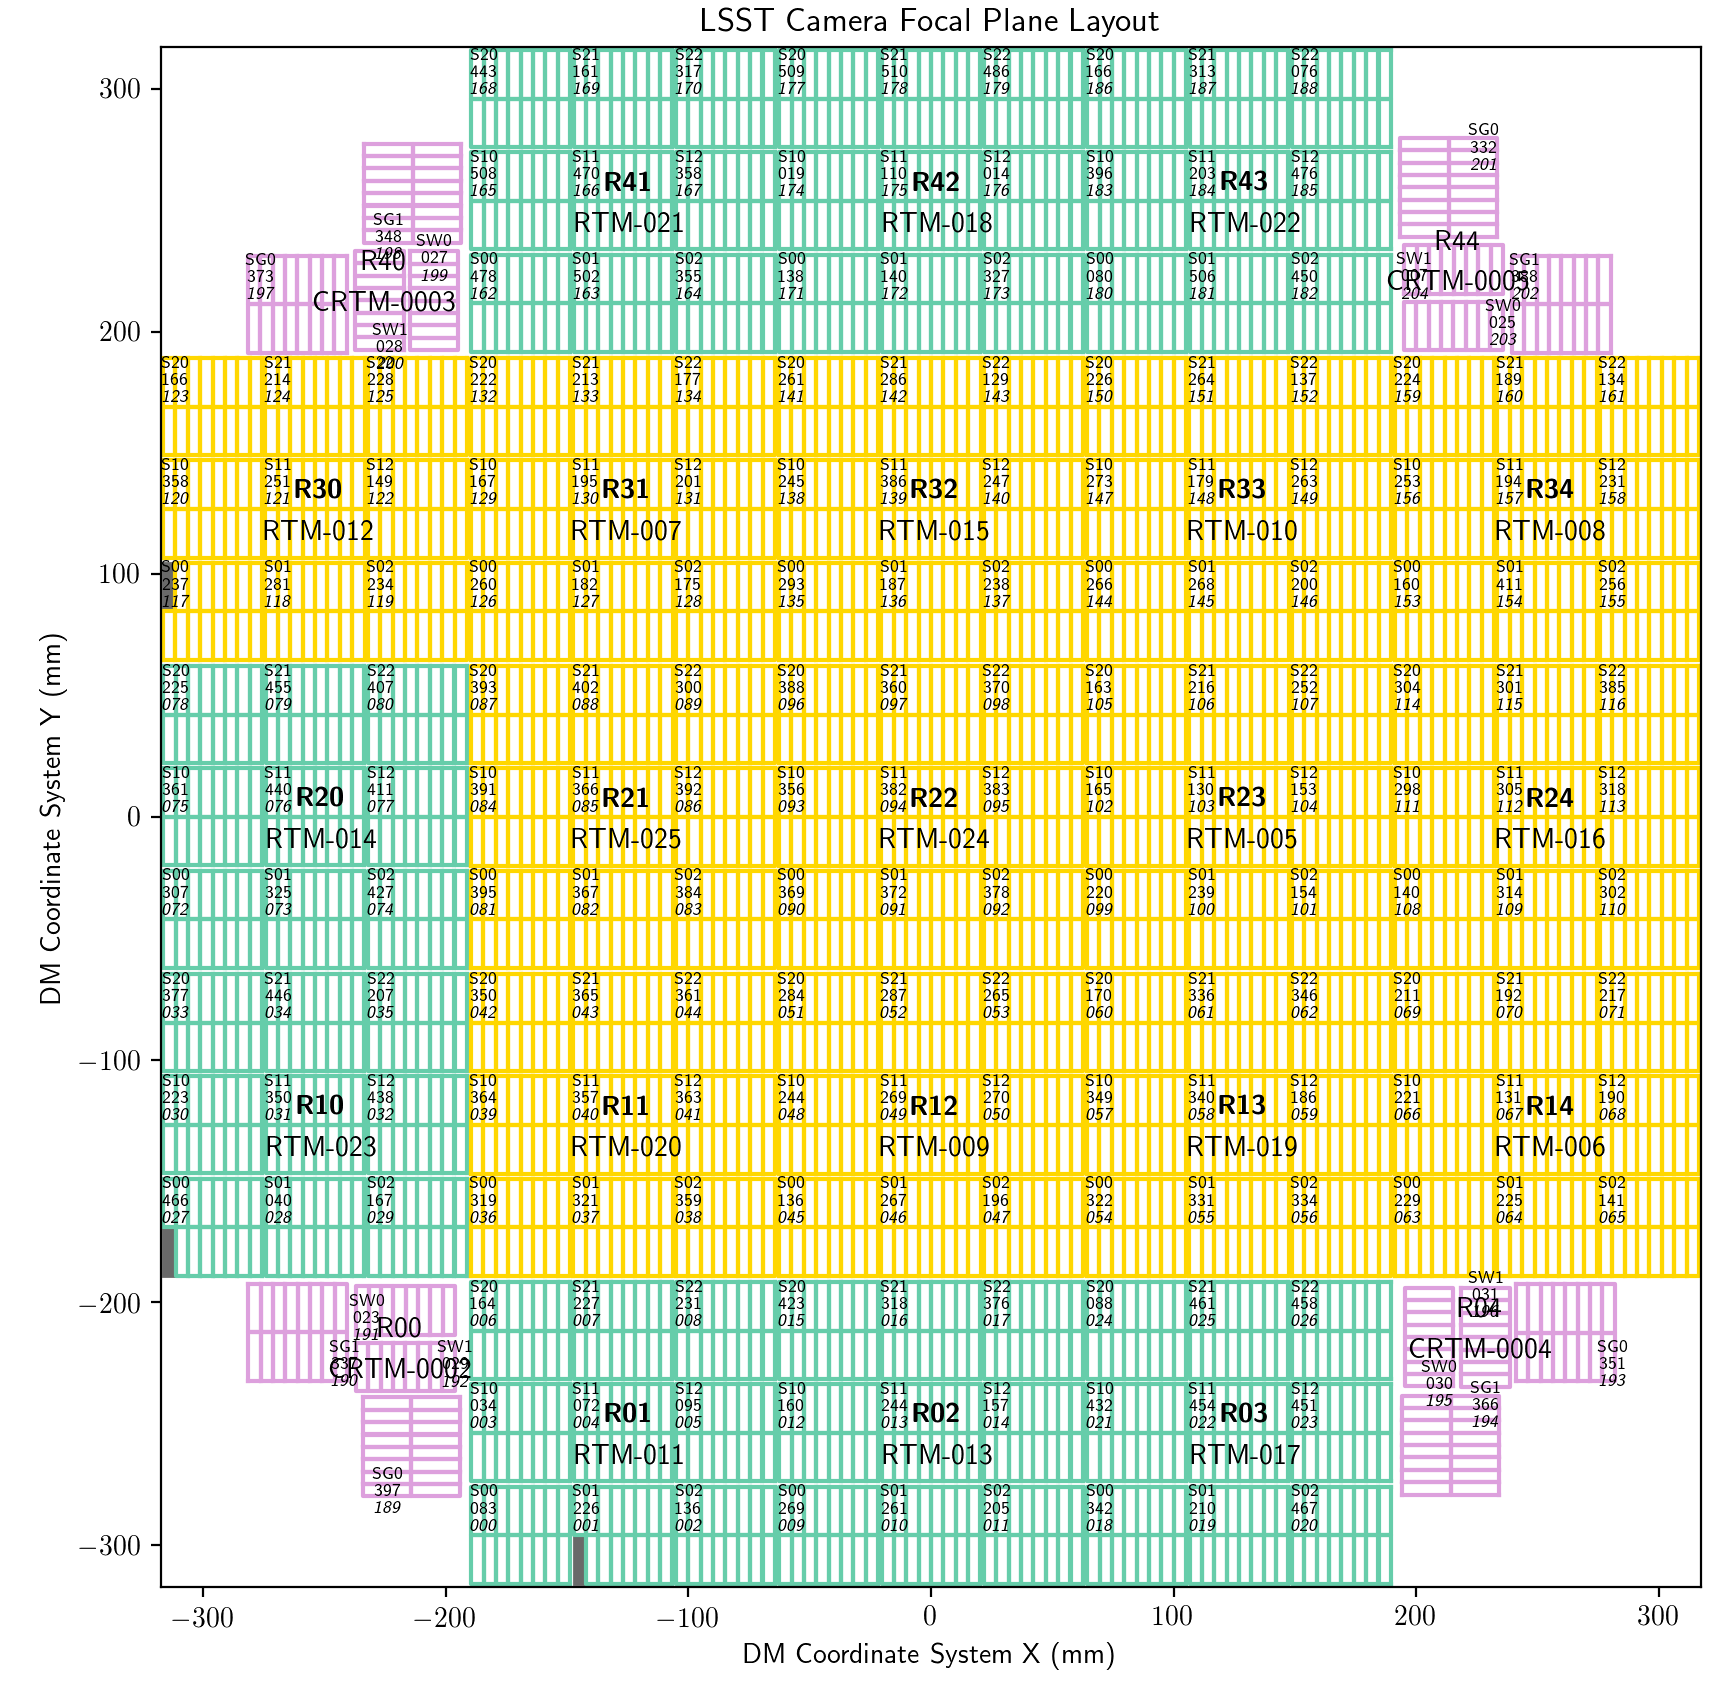
\includegraphics[width=\textwidth]{Figures/FP_layout_DM.png}
    \caption{The focal plane of the LSST camera. The vendor's CCDs' location is blue for ITL and yellow for E2V. Each CCD (a small square) is composed of 16 segments, each with its amplifier, and 189 CCDs are responsible for taking the science data. The CCDs at the corners are for focusing and synchronization with the Earth's rotation (see \href{https://www6.slac.stanford.edu/news/2020-09-08-sensors-world-largest-digital-camera-snap-first-3200-megapixel-images-slac.aspx}{LSST-SLACLab}). \textit{Image credits: Seth Digel/LSST Camera project.}}
    \label{fig:FP_LSSTCam}
\end{figure}

\subsection{What is Photon Transfer Curve (PTC)?}
The Photon Transfer Curve (PTC) is a characterization tool used to determine the fundamental parameters of a CCD, such as the gain, which represents the relationship between the electrons recorded by each pixel and their conversion to Analog-to-Digital Unit (ADU). The PTC also measures the nonlinearity of the camera and its Full Well Capacity (FWC). The gain is a crucial parameter as it impacts other vital parameters like read noise, quantum efficiency, dark current, and more, making it essential for a comprehensive understanding of CCD performance \citep{2006SPIE.6276E..09D}.

Figure \ref{fig:PTC} shows the PTC of segment C06 of sensor 22 of the LSSTCam. It is evident that at low fluxes, the variance is low and increases with the flux, but not linearly, until reaching the saturation point or FWC, which is $83000$ ADU for this detector. Beyond this point, the variance begins to decrease, indicating that the flux stored in each pixel of this amplifier starts to homogenize. This nonlinear behavior is exhibited by \textit{thick fully-depleted CCDs} as explained by \cite{2006SPIE.6276E..09D}, where charge storage in a pixel is the main cause for the deviation from the expected relationship between variance and mean number of counts in a pixel, especially in flat images \citep{2015JInst..10C5015W}. The effective area of the pixel changes with the amount of charge, decreasing as the charge accumulated in the pixel increases. As a result, very bright sources are mainly affected by this phenomenon known as the BF effect. If the pixels of the CCD segment were independent, they could be described by Poisson statistics, and the PTC would follow the green line in the figure.

\begin{figure}[!htb]
    \centering
    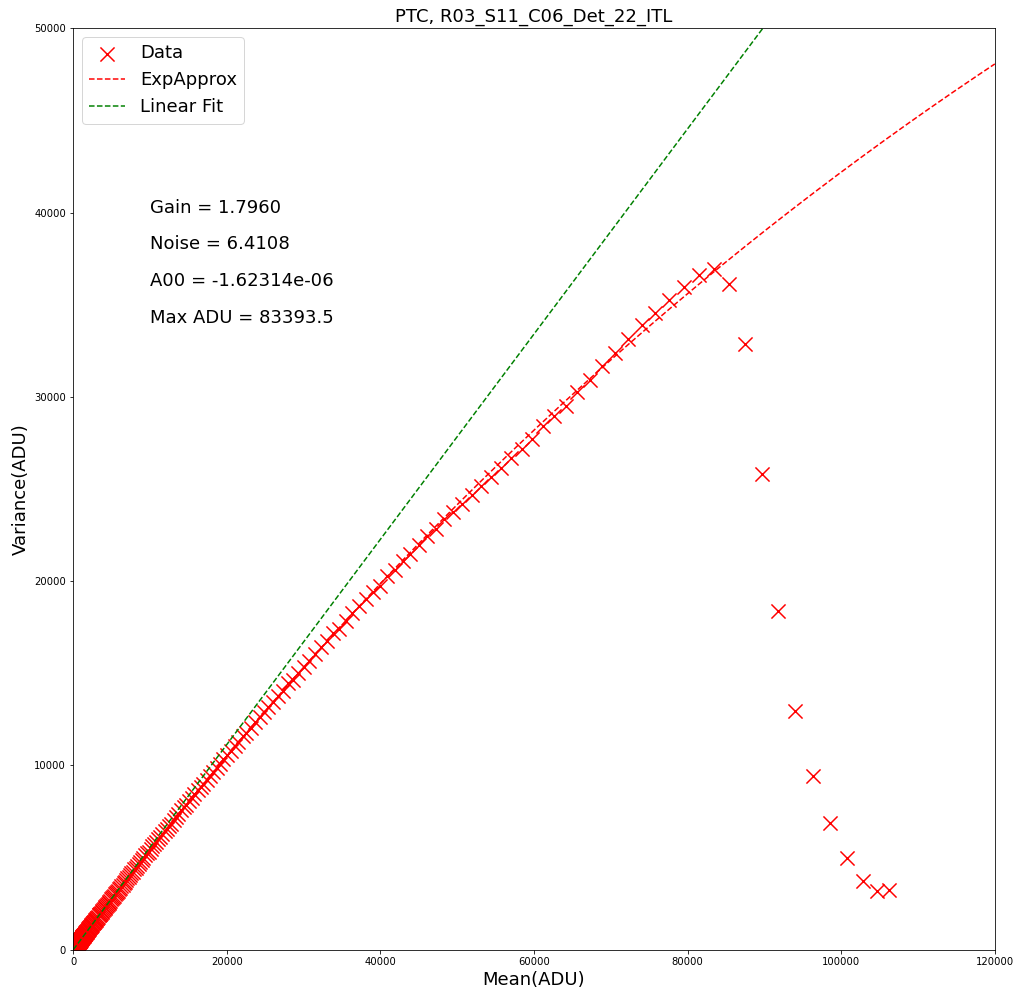
\includegraphics[width=0.7\textwidth]{Figures/PTC_R03_S11_C06_Det22.png}
    \caption{Photon Transfer Curve (PTC) for detector 22, which is located in raft 03, sensor 11, and amplifier C06, and manufactured by ITL. The red crosses represent the data points, the red line shows the EXPAPPROXIMATION fit, and the green line represents the linear fit. This PTC curve was generated using the results obtained via the \textit{DM stack}.}
    \label{fig:PTC}
\end{figure}

\subsubsection{Brigther father effect}

As mentioned previously, the charge stored in a pixel can alter the effective area of the pixel, reducing the probability that the pixel will continue to store the charge. This can result in horizontal deflection of the electrons, causing more elliptical images. This phenomenon breaks down the initial assumption of Poisson statistics and independent charge storage in each pixel, thereby modifying the relationship between the variance and the mean number of counts per pixel \citep{2015JInst..10C5015W}. This effect can impact the Point Spread Function (PSF) and may pose a potential problem for surveys that are interested in studying variations in brightness and shape of objects \citep{2018AJ....155..258C}.

\vspace{6mm}
This work was conducted during the RECA (Red de Estudiantes Colombiana de Astronomía) internship program in 2022\footnote{The RECA internship program is a scientific research training program in Astronomy, Astrophysics, and Cosmology for students from Colombian institutions. Program website: \href{https://recastronomia.github.io/internship/}{https://recastronomia.github.io/internship/}}. The program spanned three months and also involved other activities such as remote astronomical observations at the Teide Observatory\footnote{\href{https://www.iac.es/es/observatorios-de-canarias/observatorio-del-teide}{https://www.iac.es/es/observatorios-de-canarias/observatorio-del-teide}}.

In this report, we present the data used in Section \ref{sec:data}, describe the methodology in Section \ref{sec:methods}, present the results and analysis in Section \ref{sec:results}, and provide conclusions in Section \ref{sec:conclusions}."

\section{Data} \label{sec:data}

The data used in this work were obtained using the Bench for Optical Testing (BOT), which was built and designed at SLAC National Accelerator Laboratory. BOT allows laboratory tests with the LSSTCam with variations of less than 5 \% in flat images so that measurements of the linearity, full well, and gain of the PTCs can be made \citep{newbry2018lsst}. Figure \ref{fig:BOT_stand} shows the structure of the BOT, where the cryostat is located in the circular top and the focal plane is pointing down the test bench. 

%Los datos utilizados en este trabajo fueron obtenidos mediante el banco de pruebas Bench for Optical Testing (BOT), que fue construido  y diseñado en SLAC National Accelerator Laboratory, el cual permite realizar pruebas de laboratorio con la LSSTCam con variaciones menores a 5\% en imágenes flat de modo que puedan efectuarse medidas de la linealidad, full well y la ganancia de las PTC \citep{newbry2018lsst}. En la figura \ref{fig:BOT_stand} se muestra la estructura del BOT, donde en la parte superior circular va el criostato y el plano focal queda apuntando hacía abajo del banco de pruebas. 


\begin{figure}[!htb]
    \centering
    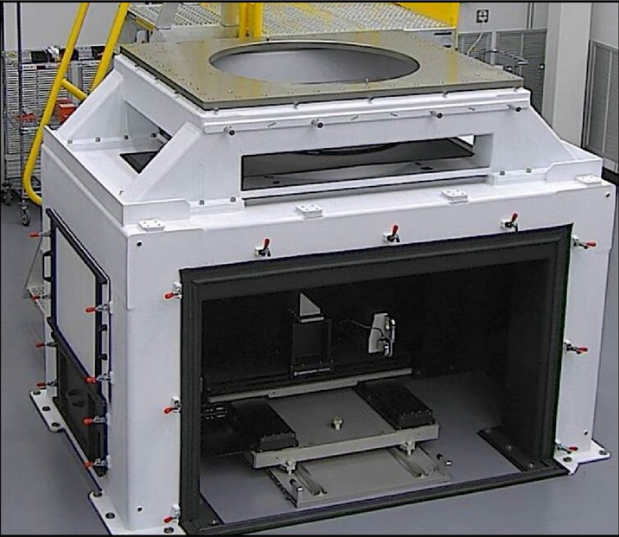
\includegraphics[width=0.7\textwidth]{Figures/BOT_stand.png}
    \caption{Bench for Optical Testing (BOT) designed by SLAC. Figure is taken from \cite{newbry2018lsst}. }
    \label{fig:BOT_stand}
\end{figure}

The \textit{run 13144} and \textit{run 13186} were used, the latter containing the crosstalk matrix information. According to \cite{snyder2020laboratory}, the electronic crosstalk measurements are carried out using a projector called \textit{crosstalk projector}, which illuminates a single sensor with a pattern of large bright spots with a collimated beam of light, which has a radius of 80 pixels. However, to perform laboratory tests simulating real source sizes they used the optical projector called \textit{the spot grid projector}. This projector generates spots in specific grids and has filters that simulate both lines left by satellites and the signal level of the sky background.

%Se hizo uso de los \textit{run 13144} y \textit{run 13186}, siendo este último el que contiene la información de la matriz de crosstalk. De acuerdo con \cite{snyder2020laboratory} las mediciones del crosstalk electrónico es llevado a cabo mediante un proyector llamado \textit{proyector crosstalk}, el cual ilumina un solo sensor con un patrón de grandes puntos brillantes con un haz de luz colimado, que posee un radio de 80 pixeles. Sin embargo, para hacer las pruebas de laboratorio simulando tamaños de fuentes reales se utiliza el proyector óptico llamado \textit{the spot grid projector}, que genera puntos en grids específicos y cuenta con filtros que simulan tanto líneas dejadas por satélites, como el nivel de señal del fondo del cielo.
\section{Methodology} \label{sec:methods}

The images used in this study underwent standard reduction techniques, including overscan, bias, dark, and defects reduction. Defects reduction involves creating maps that indicate regions with both bright and dark defects, such as dead pixels. These reductions serve as the starting state for the PTC study. Subsequently, other corrections, such as linearity and crosstalk, are applied to analyze their effects on the main parameters of the camera.

\vspace{3mm}
Professor Craig Lage generated supercalibrations for the entire focal plane, which are stored in his personal collection at \textit{u/cslage/calib/13144/calib.20220103}. The images shown in Figures \ref{fig:superbias} and \ref{fig:superdark} are superbias and superdarks, respectively, generated as part of the learning process for producing the calibration images using the LSST's software called \textit{DM stack}.

\vspace{3mm}
The code used to generate the calibration images via \textit{DM stack} can be found at \\ \href{https://github.com/lsst/cp_pipe}{https://github.com/lsst/cp\_pipe}. This code generates the data for the construction of the PTC and calculates the gain for each CCD segment as its FWC. Additionally, it calculates the gain using another method, which was analyzed in Section \ref{subsec: method_gainflat} to determine the differences between it and the PTC method. The alternative method involves using two pairs of flats for gain estimation. We utilized two versions of the \textit{DM stack} code\footnote{The DM stack software is developed for the LSST and is publicly available on GitHub at \href{https://github.com/lsst/}{https://github.com/lsst/}} for the entire focal plane:

\begin{itemize}
    \item w\_2022\_27: Initial version we started working with.
    \item w\_20222\_32: Version that includes one of our main results on obtaining the gain with pairs of flats (see the \href{https://jira.lsstcorp.org/browse/DM-35790}{DM-35790} ticket in Jira).
\end{itemize}

BPS (Batch Processing Service) was utilized to run the two previous versions. Detailed instructions on how to build the configuration files, handle possible errors, and access more information can be found in the GitHub repository of this project, \href{https://github.com/linagiraldom/RECA_Internship_Project}{RECA\_Internship\_Project}, in the notebook \href{https://github.com/linagiraldom/RECA_Internship_Project/blob/main/Notebooks/BPS_LSST.ipynb}{BPS\_LSST.ipynb}. Additionally, all the notebooks used to carry out the methodology described below are available in this repository. There is also a tutorial notebook called \href{https://github.com/linagiraldom/RECA_Internship_Project/blob/main/Notebooks/Tutorial.ipynb}{Tutorial.ipynb}, where I provide an overview of the \textit{Data Butler}, the API that manages and stores the data. It includes information on collections, image visualization, data retrieval, and other details related to the calibration images.

\begin{figure}[!htb]
     \centering
     \begin{subfigure}[b]{0.49\textwidth}
         \centering
         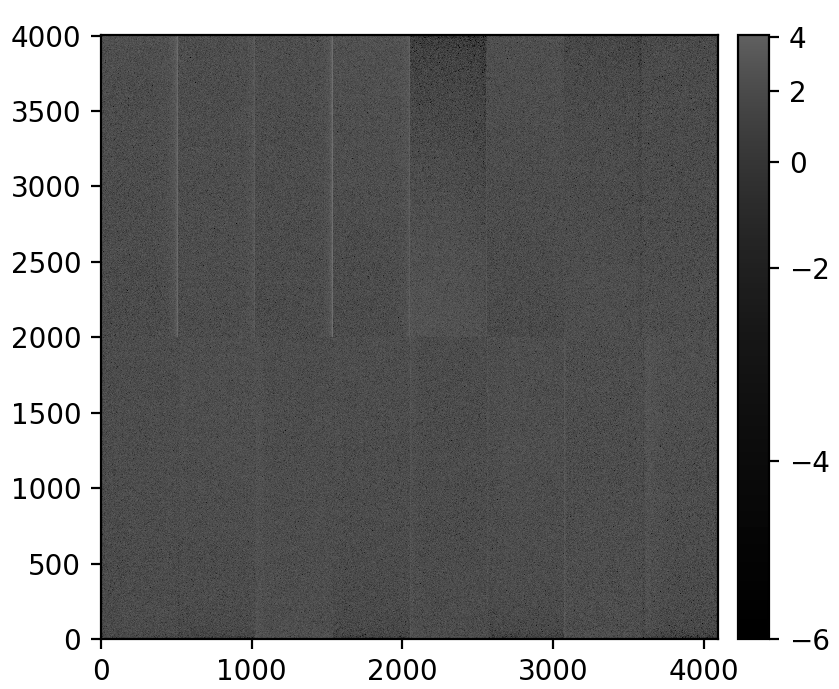
\includegraphics[width=\textwidth]{Figures/Super_bias_55.png}
     \end{subfigure}
     \hfill
     \begin{subfigure}[b]{0.49\textwidth}
         \centering
         
\includegraphics[width=\textwidth]{Figures/Super_bias_74.png}
     \end{subfigure}
        \caption{Masterbias images for detectors 55 (E2V) on the left and 74 (ITL) on the right.}
        \label{fig:superbias}
\end{figure}

\begin{figure}[!htb]
     \centering
     \begin{subfigure}[b]{0.49\textwidth}
         \centering
         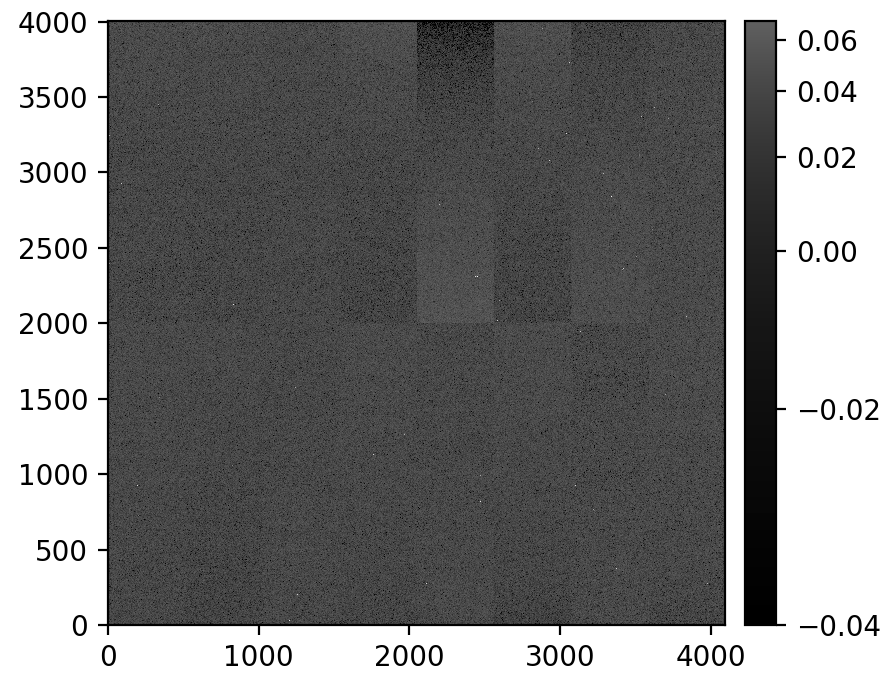
\includegraphics[width=\textwidth]{Figures/Super_dark_55.png}
     \end{subfigure}
     \hfill
     \begin{subfigure}[b]{0.49\textwidth}
         \centering
         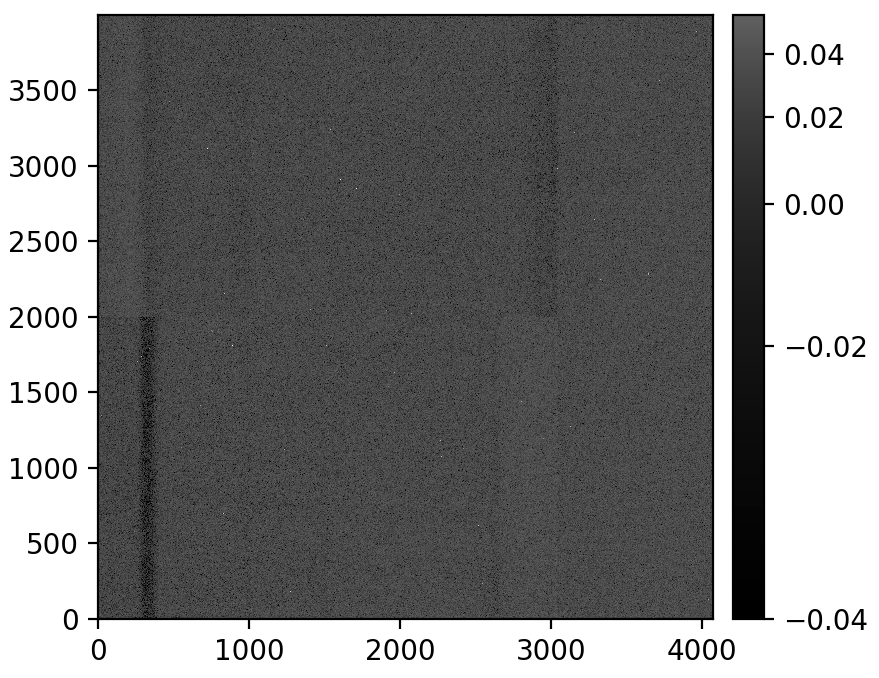
\includegraphics[width=\textwidth]{Figures/Super_dark_74.png}
     \end{subfigure}
        \caption{Masterdarks images for detectors 55 (E2V) on the left and 74 (ITL) on the right}
        \label{fig:superdark}
\end{figure}


\subsection{Photon Transfer Curve (PTC)}
The PTCs were generated for the entire LSSTCam focal plane using the \textit{DM stack}\footnote{The PTCs are constructed with the code available in the repository \href{https://github.com/lsst/cp_pipe}{cp\_pipe}}, which allows estimating the gain, read noise, $a_{00}$ (parameter related to the BF effect), and turnoff (associated with the FWC) from a fit to the shape of the PTC. This code implements equations 16 and 20 of the \cite{2019A&A...629A..36A} article: equation 16 corresponds to the exponential approximation (EXPAPPROXIMATION), which uses only the variance ($C_{00}$); while equation 20 is the full model (FULLCOVARIANCE), and implements the covariance matrix. In this work, we used EXPAPPROXIMATION, which is described by the following equation:

\begin{equation}
    C_{00} = \frac{1}{2 g^2 a_{00}} [\exp (2 a_{00} \mu g) - 1] + \frac{n_{00}}{g^2}
    \label{eq:Astier16}
\end{equation}

where $C_{00}$ is the variance, $g$ is the gain, $a_{00}$ is always negative and is related to the B-F effect, $mu$ is the mean, and $n_{00}$ ($el^{2}$) is the noise. According to \cite{2019A&A...629A..36A}, a negative value of $a_{00}$ leads to the variance of a flat field not growing as fast as the mean does. In the case where there is no BF effect, i.e., each pixel is independent of the other and is described by a Poisson statistic, the mean, gain, and variance are directly related through the equation:

\begin{equation}
    V = \frac{\mu}{g}
    \label{eq:gain_Poisson}
\end{equation}

where $V$ is the variance of a flat field, $\mu$ is the mean, and $g$ is the gain.



\subsection{Gain from flat pairs} \label{subsec: method_gainflat}
An independent method for calculating a sensor's gain is using flat field pairs with equal exposure times. Since each CCD is composed of 16 segments, each with its amplifier, a gain value is obtained for each segment. For this purpose, LSST has the function \href{https://github.com/lsst/cp_pipe/blob/main/python/lsst/cp/pipe/ptc/cpExtractPtcTask.py#L679}{Gain from flat pairs}, which was analyzed in detail in this work.

\vspace{3mm}
We aim to quantify the difference between the gain calculated from the fit to the PTC and this independent method using flat field pairs with equal exposure times. For this, we initially calculate the average flux in ADU with each flat pair, the read noise, and the gain. The latter is estimated employing the equation of \cite{2014JInst...9C4023L}:

\begin{equation}
    \frac{1}{g} = \Big \langle \frac{(I_1 - I_2)^2}{I_1 + I_2} \Big \rangle 
    \label{eq:Lupton}
\end{equation}

where $g$ is the gain, $I_1$ is the first flat image, and $I_2$ is the second flat image, both taken at the same exposure time. The expected value over all pixels is the inverse of the gain. Considering corrections for read-out noise, the equation takes the following quadratic form:

\begin{equation}
    \frac{1}{g} = \Big \langle \frac{(I_1 - I_2)^2}{I_1 + I_2} \Big \rangle - \frac{1}{\mu} (N^2-\frac{1}{2} g^2)
    \label{eq:gain_corrected}
\end{equation}

Where $\mu = 0.5(\mu_1 + \mu_2)$, with $\mu_1$ and $\mu_2$ being the average values for each of the flat images, and $N$ is the read-out noise. The equation above has three variants: NONE, SIMPLE, and FULL, with NONE being equivalent to Equation \ref{eq:Lupton}. The remaining two cases are as follows:

\begin{align}
g = \begin{cases}
  \frac{1}{K - \frac{1}{\mu}(N^2 - \frac{1}{2} g^2)} & \mbox{SIMPLE} \\
  \frac{\mu + \sqrt{\mu^2 - 2 \mu K + 2 N^2}}{2 K \mu - 2 K^2} & \mbox{FULL}
\end{cases}
\label{eq:sol_gain_corrected}
\end{align}

where $K$ is equal to Equation \ref{eq:Lupton}. In the SIMPLE case, $g = 1/K$, while in the FULL case, the quadratic equation is solved, and the result is taken to have physical meaning. Once we have the gains calculated from pairs of flats for flows between 0 and $\sim 10000$ ADU, we calculate the relative percentage error with the gain obtained from the fit to the PTC using Equation \ref{eq:sol_gain_corrected} with the FULL type correction:

\begin{equation}
    \mbox{Relative\_error} [\%] = \frac{|gain_{PTC} - gain_{flats}|}{gain_{PTC}} \times 100 \% 
    \label{eq:error_relativo_gain}
\end{equation}

Subsequently, a linear low-flow fit was performed, which we considered to be between 5000 and 10000 ADU. The low-flow fit has the following form:

\begin{equation}
    \mbox{Relative\_error}_{LF} [\%] = m F + \mbox{offset}
\end{equation}

Where $m$ is the slope of the fit, $F$ is the flux, and \textit{offset} is the intercept with the $y$-axis. These parameters are used to quantify the error variation in the specified flow range and the base error between the PTC gain and that calculated with the flats. We generated histograms of these parameters to examine the behavior of the vendor's data and extract general trends. To exclude outliers, i.e., CCD segments with abnormal behavior, we utilized the \textit{sigma\_clip} and \textit{sigma\_clipped\_stats} functions from \cite{2018AJ....156..123A}. These functions allowed us to cut the data such that only values within $3 \sigma$ of the median were retained, and we performed this operation iteratively three times to ensure robustness.


 \begin{figure}[!htb]
     \centering
     \begin{subfigure}[b]{\textwidth}
         \centering
         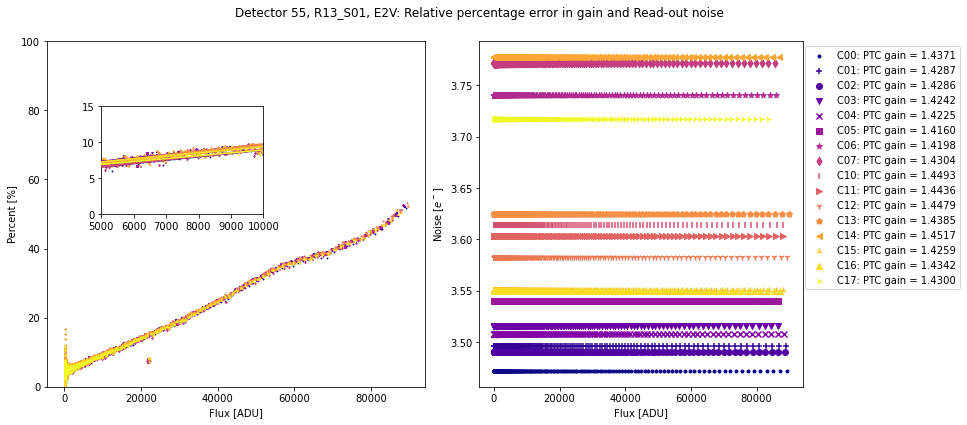
\includegraphics[width=\textwidth]{Figures/Relative_Error_Gain_Noise_detectorR13_S01_old.png}
     \end{subfigure}
     \vspace{3mm}
     \begin{subfigure}[b]{\textwidth}
         \centering
         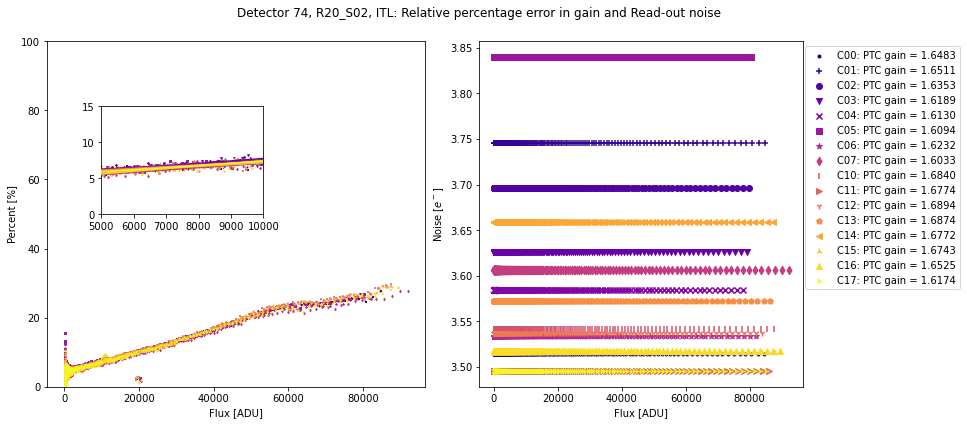
\includegraphics[width=\textwidth]{Figures/Relative_Error_Gain_Noise_detectorR20_S02_old.png}
     \end{subfigure}
        \caption{The relative percentage error between the gain estimated by the PTC and the gain calculated from two flat images is shown in the left panels, while the read-out noise of each amplifier is shown in the right panels. The upper panel displays the results for detector 55 (R13\_S01) with vendor E2V, and the lower panel shows the results for detector 74 (R20\_S02) from vendor ITL. Each color and symbol in the plots represents the relative percentage error for one of the 16 segments that make up each CCD. The embedded image in the left panels shows the percentage error specifically between 5000 and 10000 ADU, corresponding to the low flux regime where a linear fit is performed. The data used to construct these plots includes only values below the PTC turnoff.}
        \label{fig:relative_error_oldcode}
\end{figure}


\begin{figure}[!htb]
    \centering
    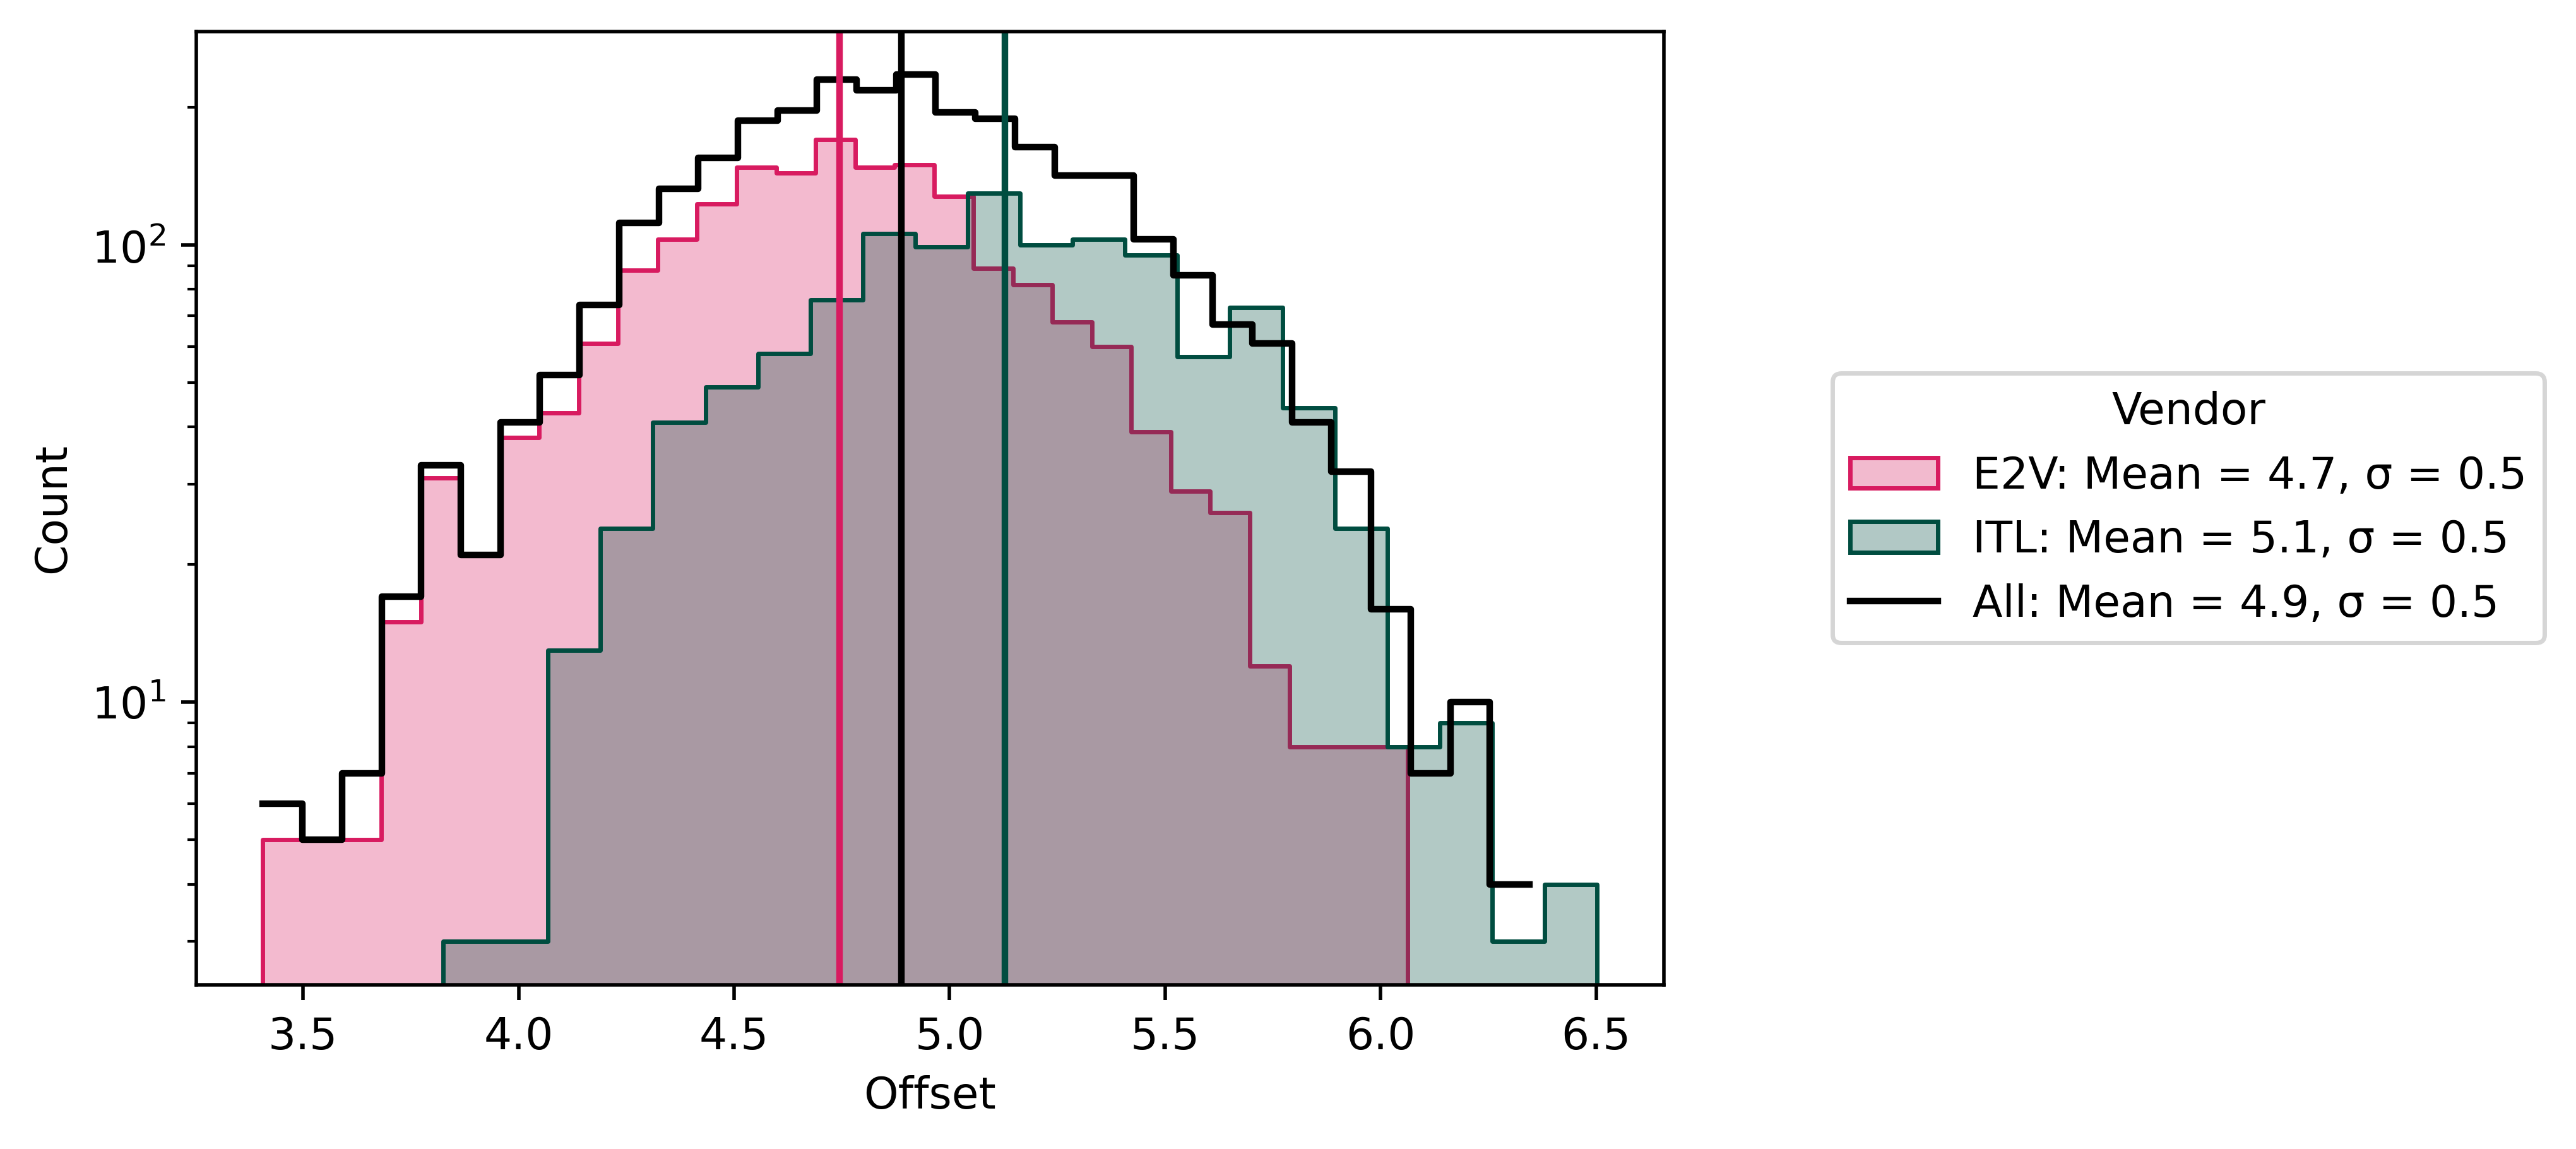
\includegraphics[width=\textwidth]{Figures/Histogram_offset_old.png}
    \caption{The histograms display the offset value obtained from the linear fit for flows between 5000 and 10000 ADU, representing the relative percentage error between gains. The magenta distribution represents the results for vendor E2V, with a mean of $(4.7 \pm 0.5)$ \%. The blue distribution shows the results for vendor ITL, with a mean of $(5.1 \pm 0.5)$ \%. The black distribution represents the histogram of all data without discrimination by vendor, with a mean of $(4.9 \pm 0.5)$ \%. Vertical lines indicate the value of the mean for each distribution.}
    \label{fig:hist_offset_old}
\end{figure}

\subsubsection{Simulation} \label{subsubsec:method_Simulation_Gain}

The methodology outlined in Section \ref{subsec:method_gainflat} and the utilization of LSST software version \textit{w\_2022\_27} yielded the results depicted in Figures \ref{fig:relative_error_oldcode} and \ref{fig:hist_offset_old}. Figure \ref{fig:relative_error_oldcode} showcases the relative percent error between the gains for E2V sensor 55 (top panel) and ITL sensor 74 (bottom panel) over the flow range below the PTC turnoff. The embedded plot on the left displays the behavior between 5000 and 10000 ADU, along with the corresponding linear fit, while the plot on the right shows the error for each CCD segment within the same flow range. Notably, the embedded plot reveals that the relative error has an offset exceeding 5\% for these two sensors, prompting us to construct a histogram with the offset values for the entire focal plane to determine if this behavior is widespread. Figure \ref{fig:hist_offset_old} confirms that this relative error is a prevalent characteristic exhibited by all sensors, with an average base error of $\sim 5$\%, which we consider relatively high. Thus, we further investigated this issue through simulations.

\vspace{3mm}

Various factors, including potential overestimation of the read-out noise, the influence of masks used in the images, or assumptions about the distribution for the operations between flat images as given by Equation \ref{eq:ratioIm}, could contribute to the observed behavior. The \textit{w\_2022\_27} version of the \textit{DM stack} assumes that Equation \ref{eq:ratioIm} follows a Gaussian distribution.

\begin{equation}
      \frac{(I_1 - I_2)^2}{I_1 + I_2} 
      \label{eq:ratioIm}
\end{equation}

To better understand and address this issue, further analysis and simulations were conducted. If the distribution is found to deviate from a Gaussian distribution, the distribution statistics would need to be modified accordingly. To explore possible variables, we conducted simulations in three different cases, as described below:


\begin{itemize}
    \item \textbf{Case 1 - Noise Overestimation}: Two data sets were constructed following a Poisson distribution for the flow, with an expected value ranging from 5000 to 10000 ADU. In our case, we chose 5000 ADU as the expected value. The Poisson distribution is given by:
 
    \begin{equation}
        f(k;\lambda) = \frac{\lambda^k e^{-\lambda}}{k!} \implies f(k;5000) = \frac{5000^k e^{-5000}}{k!}
    \end{equation}
    \label{eq:dist_Poisson}

    where $\lambda$ is the expected value and $k$ is the number of events. To this data, we added Gaussian noise with a mean of zero and a dispersion value that we assume as the read-out noise, given by:
    
    \begin{equation}
        p(x) = \frac{1}{\sqrt{2 \pi \sigma^2}} \exp \Big(-\frac{(x - \mu)^2}{2\sigma^2} \Big) \implies p(x) = \frac{1}{\sqrt{2 \pi N^2}} \exp \Big(-\frac{x^2}{2N^2} \Big)
        \label{eq:gaussian_noise}
    \end{equation}
    
    where $\mu$ is the mean, $\sigma$ is the standard deviation, and $N$ is the read-out noise that we assume. Finally, we apply the methodology described in Section \ref{subsec: method_gainflat} for all types of gain correction: NONE, SIMPLE, and FULL, and calculate the relative error using a base gain (chosen as 2.0) to verify if we can replicate the observations in Figure \ref{fig:relative_error_oldcode}, specifically a base error above 5\%.

    \item \textbf{Case 2 - Pixel Masks}: In this step, pixel masks are added to Case 1. The respective mask is extracted from each flat image, where each flat has an average of 5000 ADU counts. This mask filters out suspicious, bad, dead, and saturated pixels. Next, a Poisson distribution is generated with the dimensions of one of the CCD segments for which the masks were extracted, i.e., $size_x = 2002$ and $size_y = 512$, along with its respective Gaussian noise. The generated mask is then applied to each array using the \textit{Numpy} function \citep{2020Natur.585..357H} \textit{ma.masked\_where}.

    
    \begin{figure}[!htb]
        \centering
        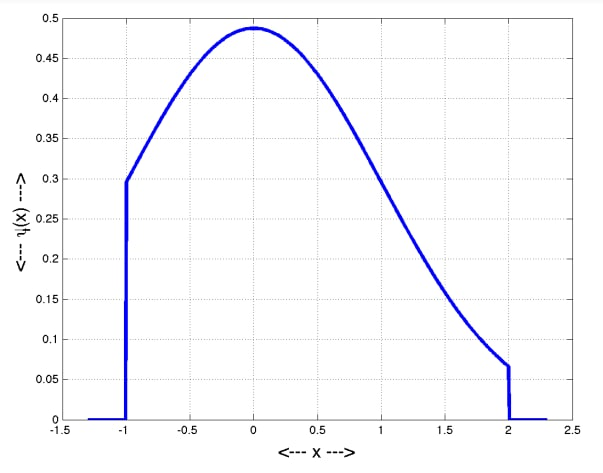
\includegraphics[width=0.5\textwidth]{Figures/Truncated_Gaussian.jpg}
        \caption{The truncated Gaussian distribution with a zero mean and standard deviation is represented by $\psi(0,1,a = -1, b = +2; x)$. This figure is sourced from \cite{burkardt2014truncated}.}
        \label{fig:truncated_gaussian_dist}
    \end{figure}

    \textbf{Case 3 - Statistics control}: Building upon Case 2, we incorporate statistics control by assuming that the distribution of equation \ref{eq:ratioIm} follows a Gaussian distribution. Similar to the approach used in section \ref{subsec:method_gainflat}, we truncate the distribution by keeping only the data points that fall within $5.5 \sigma$ of the mean, and we repeat this process for three iterations. When the distribution of equation \ref{eq:ratioIm} is Gaussian, the mean of the symmetrical truncated distribution is the same as the original one, and the mean of non-symmetrical truncated distribution can be calculated as:
    
    \begin{equation}
        \mu = \overline{\mu} - \overline{\sigma} \frac{\phi (0,1; \beta) - \phi (0,1; \alpha)}{\Phi (0,1; \beta) - \Phi (0,1; \alpha)} \; \; \; ; \alpha = \frac{a-\overline{\mu}}{\overline{\sigma}} , \beta = \frac{b -\overline{\mu}}{\overline{\sigma}}
        \label{eq:truncated_dist}
    \end{equation}

    where $\alpha$ and $\beta$ are standardized variables, $a$ and $b$ are the cutoff values for the lower and upper tails of the distribution, respectively, $\overline{\mu}$ and $\overline{\sigma}$ are the statistics of the original distribution, $\phi$ represents the normal probability density function (PDF), and $\Phi$ represents the Normal cumulative distribution function (CDF). Figure \ref{fig:truncated_gaussian_dist} illustrates this case for $a=-1$ and $b=+2$. However, when the distribution is symmetrically truncated, i.e., $-a=b$, the numerator of the second term in the above equation becomes zero, and the mean of the truncated and original distribution is simply:
    
    \begin{equation}
        \mu = \overline{\mu}
        \label{eq:truncated_dist_simetric}
    \end{equation}

    This implies that the mean of the truncated and original distribution are equal, as mentioned earlier. We use this result to calculate the expected value of equation \ref{eq:Lupton} in order to determine the gain solutions for the NONE, SIMPLE, and FULL corrections. As an additional step, we examine the shape of the distribution of equation\ref{eq:ratioIm}; if the distribution of equation \ref{eq:ratioIm} is not Gaussian, no truncation is applied, and the expected value of equation \ref{eq:Lupton} is calculated using the arithmetic mean.

\end{itemize}


\subsection{No linearity Correction} \label{subsec:method_Linearity}

To study the impact of linearity correction on the PTC shape and parameters, we applied a Spline linearizer with 12 nodes to detectors 32 (ITL) and 139 (E2V). This linearizer was generated by Jerónimo\footnote{Jerónimo was my partner during this internship, who worked on the sister project \textit{Study of the Linearity of the CCDs of the Vera C. Rubin Observatory}} \citedsp{RTN-055}, who found in his analysis that a Spline with 12 equally spaced nodes significantly corrects the nonlinearity effect and reduces dispersion in the residuals. All configurations remained unchanged, except for the linearity correction (see table \ref{tab:config_linearity}).


\begin{table}[!htb]
\centering
\caption{The configuration used to generate the PTCs when we include the linearity correction (the parameter 'doLinearize' is set to 'true').}
\label{tab:config_linearity}
\resizebox{\textwidth}{!}{%
\begin{tabular}{cccc}
\hline
\multicolumn{4}{c}{\textbf{Configurations}} \\
\hline
\hline
  doWrite: true       &  doLinearize: true      &  doFlat: false       &  doInterpolate: false  \\
  doOverscan: true    &  doCrosstalk: false      &  doFringe: false     &  doSaturation: false   \\
  doAssembleCcd: true &  doBrighterFatter: false &  doApplyGains: false &  doSaturationInterpolation: false  \\
  doBias: true        &  doDark: true            &  doDefect: true      &  growSaturationFootprintSize: 0 \\
  doVariance: true    &  doStrayLight: false     &  doNanMasking: true  &  ptcFitType: EXPAPPROXIMATION \\
  \hline
\end{tabular}%
}
\end{table}

Subsequently, plots of the ratio of Variance to Mean vs Mean are constructed, normalizing the variance. This allows for analysis of whether the bump between 50000 and 60000 ADU is corrected. Additionally, a relative percentage error between the parameters obtained from the PTC fit with and without linearity correction is calculated to quantify the effect on these parameters. Finally, a comparison is made to check if the parameters and/or the shape of the PTC changed compared to the version without correction for nonlinearity.


\subsection{Crosstalk Correction} \label{subsec:method_Crosstalk}

The LSSTCam's full focal plane can be read out in 2 seconds, and the combination of high-speed, high-resistivity silicon components and close spacing between each channel makes it more susceptible to electronic crosstalk compared to other mosaic cameras \citep{2015JInst..10C5010O}.

\vspace{3mm}

\begin{figure}[!htb]
    \centering
    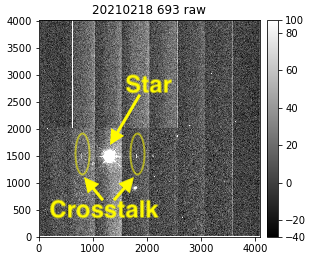
\includegraphics{Figures/Crosstalk_effect.png}
    \caption{An image of a bright star captured with the 1.2m auxiliary telescope at the Vera Rubin Observatory, revealing crosstalk in segments adjacent to the star's image.}
    \label{fig:crosstalk}
\end{figure}

Electronic crosstalk occurs in CCDs with multiple channels that are read simultaneously and coupled, resulting in ghost images generated in adjacent segments when a bright source is detected in a channel due to this coupling \citep{2020SPIE11454E..39S}. This effect is illustrated in Figure \ref{fig:crosstalk}, where ghost signals are observed in the lateral segments of the detector. Figure \ref{fig:crosstalk_matrix} shows a heat map on the left for ITL detector 32 and on the right for ITL detector 139, depicting the crosstalk coefficients in blue colors, with the observation that the crosstalk pattern differs per vendor. These coefficients are incorporated into a configuration file in the LSST software to regenerate the PTC with this correction.

Finally, similar to the approach in Section \ref{subsec:method_Linearity}, a comparison was made to check whether the parameters and/or the shape of the PTC changed compared to the version without correction for crosstalk.


\begin{figure}[!htb]
     \centering
     \begin{subfigure}[b]{0.49\textwidth}
         \centering
         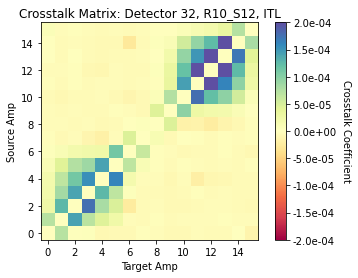
\includegraphics[width=\textwidth]{Figures/Crosstalk_32.png}
     \end{subfigure}
     \hfill
     \begin{subfigure}[b]{0.49\textwidth}
         \centering
         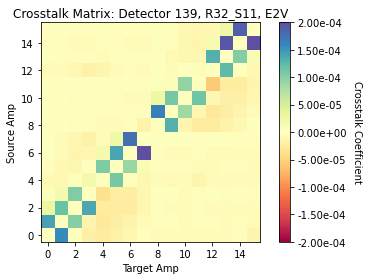
\includegraphics[width=\textwidth]{Figures/Crosstalk_139.png}
     \end{subfigure}
        \caption{Crosstalk matrix shown on the left for detector 32 (ITL) and on the right for detector 139 (E2V).}
        \label{fig:crosstalk_matrix}
\end{figure}
\section{Results} \label{sec:results}


\subsection{PTC}

As part of this project, an initial and fundamental task was to use the PTC to determine the essential parameters of each CCD segment across the focal plane, using the \textit{DM stack}. This has already been done by SLAC National Acceleration Laboratory \footnote{El código utilizado por \textit{SLAC} está disponible en \href{https://github.com/lsst-camera-dh/eotest/blob/32c17b0a33b9c099651ed581ee90c1b1101012fb/python/lsst/eotest/sensor/ptcTask.py}{SLAC code}} (hereafter SLAC) for this very run (\href{https://srs.slac.stanford.edu/BOT_EO_Reports/13144/}{SLAC heat maps BOT 13144}) and here we seek to reproduce their results.



\vspace{3mm}

%%%%%%%%%%%%Figura

\begin{figure}[!htb]
    \centering
    \includegraphics[width=\textwidth]{Figures/PTC_Detector55.png}
    \caption{PTC for all segments of sensor 55 (E2V). Xs represent the data, the red line is the fit to the PTC by exponential approximation (eq. \ref{eq:Astier16}), and the green line is a linear fit. The parameters obtained from the fit to the PTC are the gain, the $a_{00}$ parameter, the PTC turnoff (Max ADU), and the read noise. }
    \label{fig:PTC_55}
\end{figure}

%%%%%%%%%%%%%%%%%%

Initially, we generated the PTCs by CCD for the entire focal plane, as shown in Figure \ref{fig:PTC_55}, to detect PTCs with abnormal behavior and low PTC-turnoff (below 40000 ADU). Detectors found with low PTC-turnoff and/or misclassified are recorded in the table \ref{tab:PTC_warnings}. In addition, a visual inspection showed that about 60 \% of the detectors have at least one segment showing \textit{Downing dip}. 

\vspace{3mm}
%%%%%%%%%%%%Figura

\begin{figure}[!htb]
 \centering
     \begin{subfigure}[b]{0.49\textwidth}
         \centering
         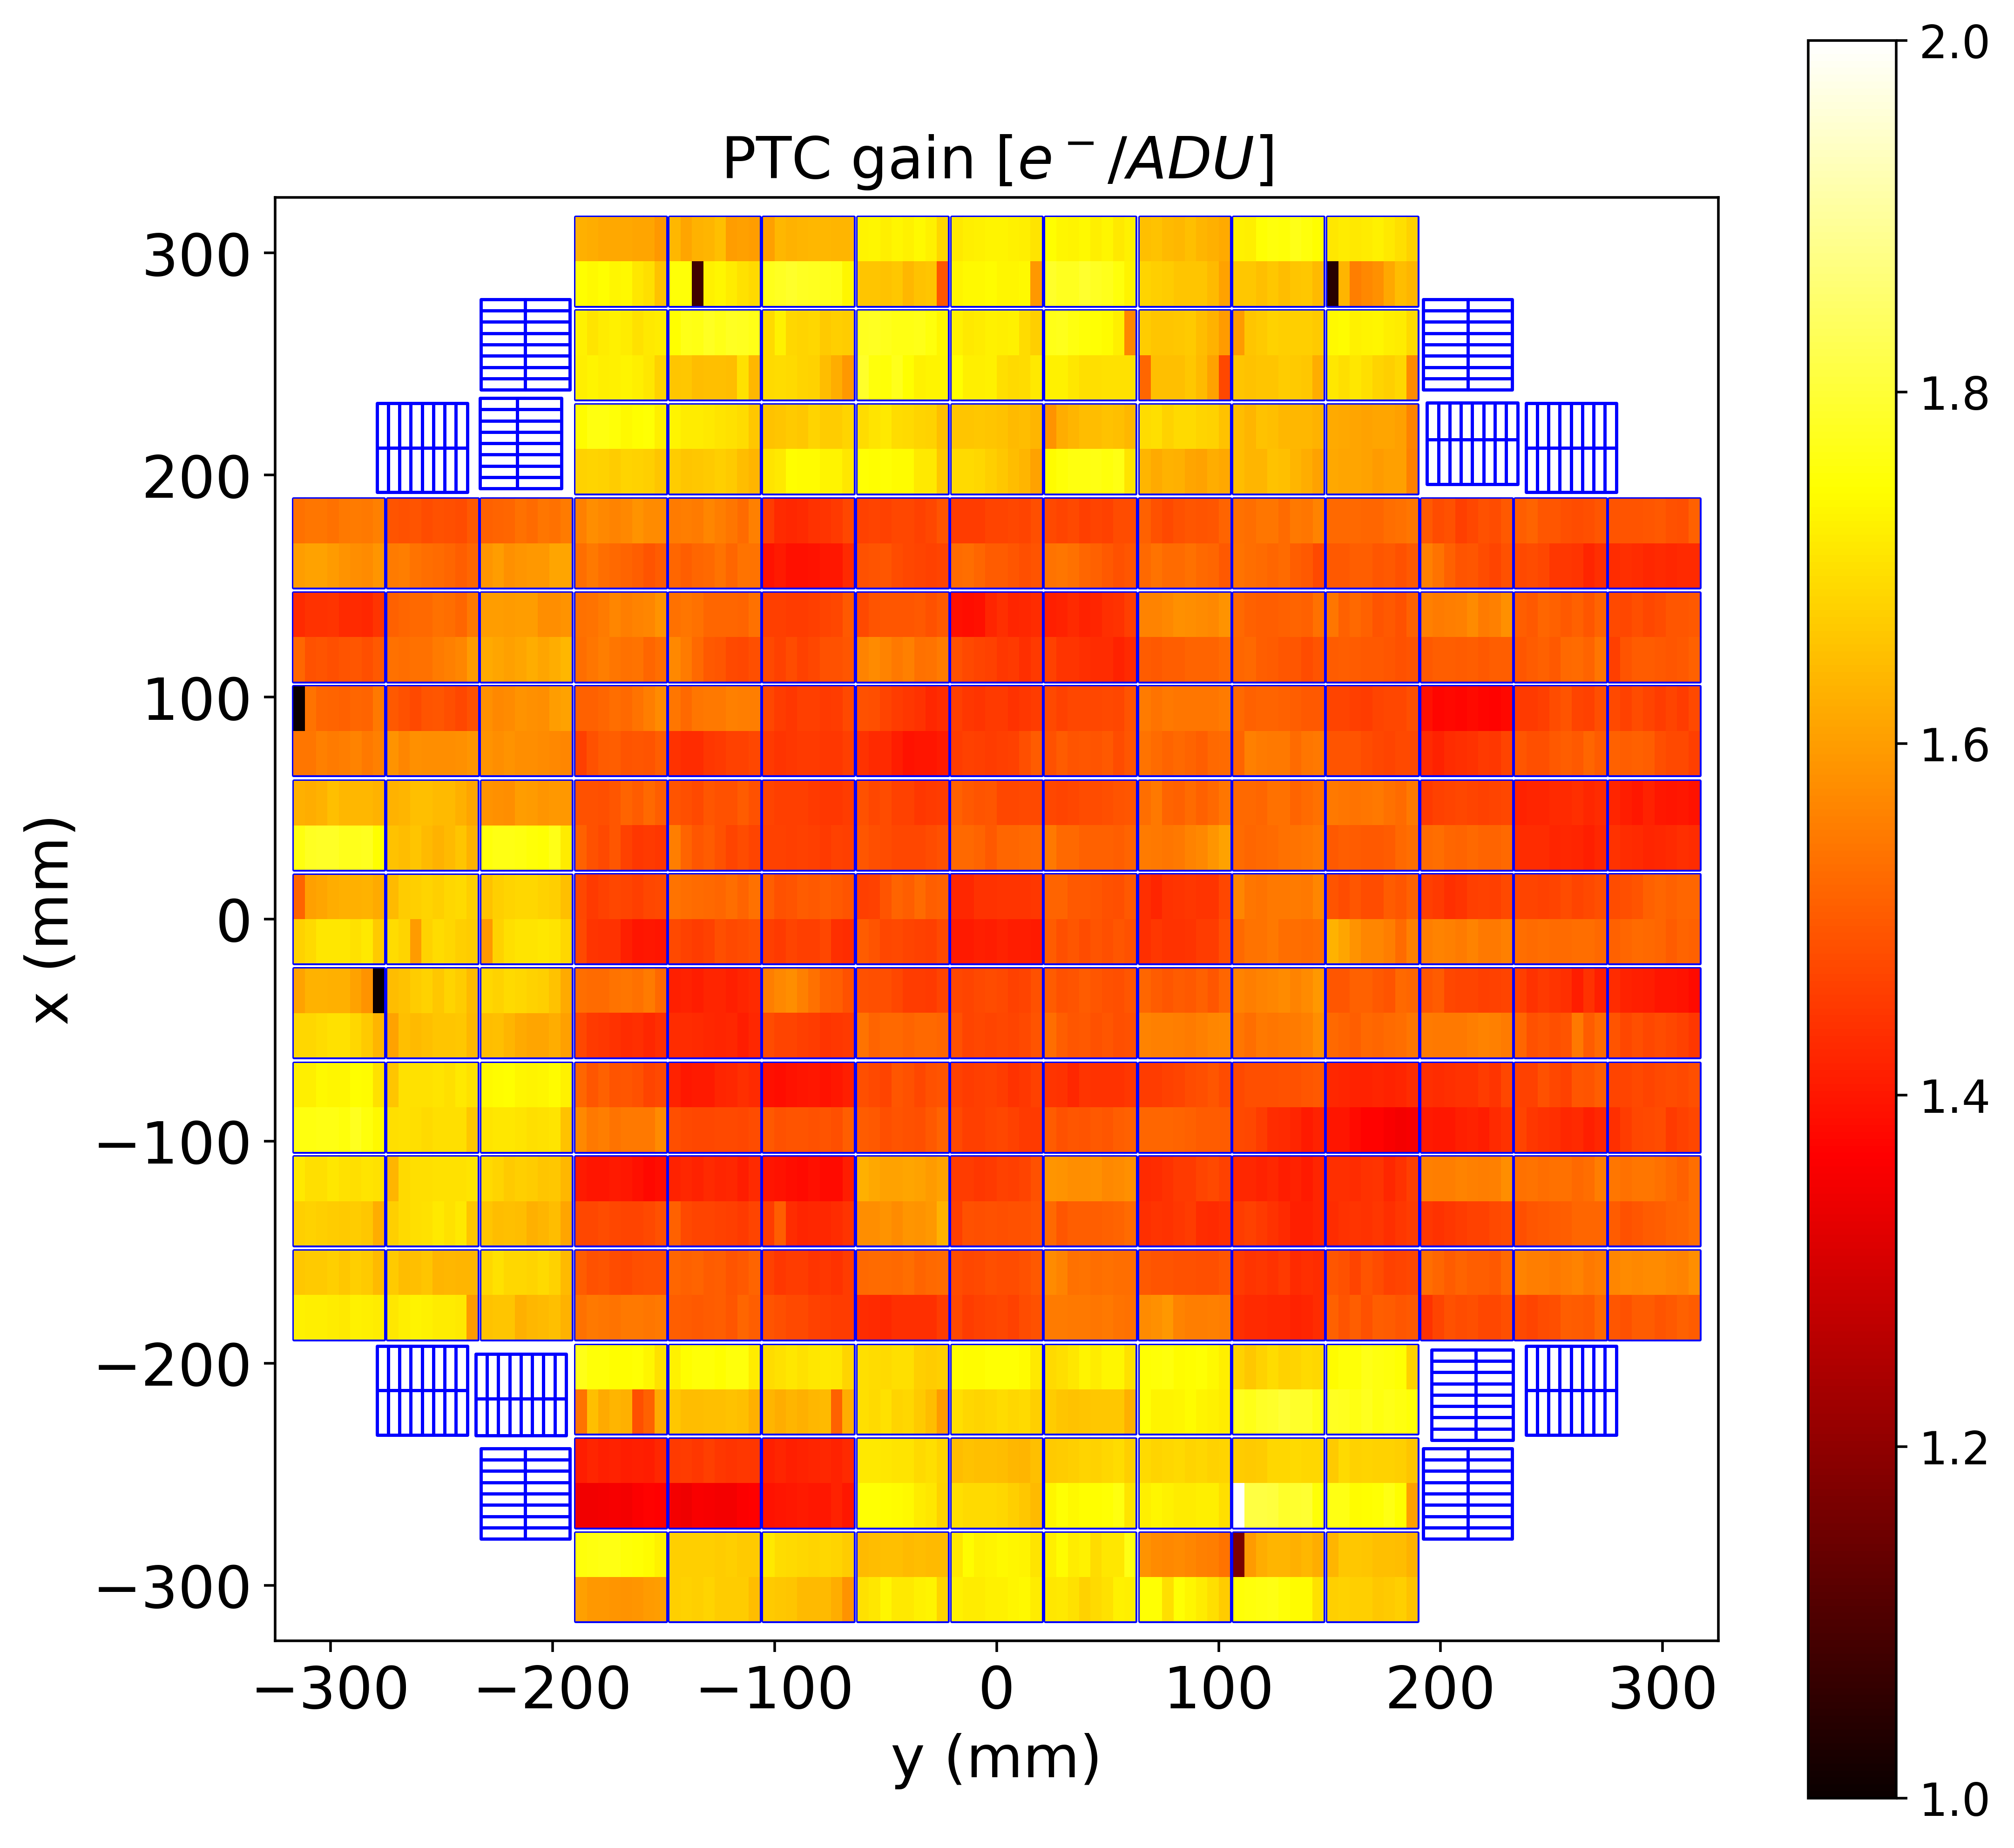
\includegraphics[width=\textwidth]{Figures/Focal_plane_gain.png}
     \end{subfigure}
     \hfill %\hspace{-10em}
     \begin{subfigure}[b]{0.49\textwidth}
         \centering
         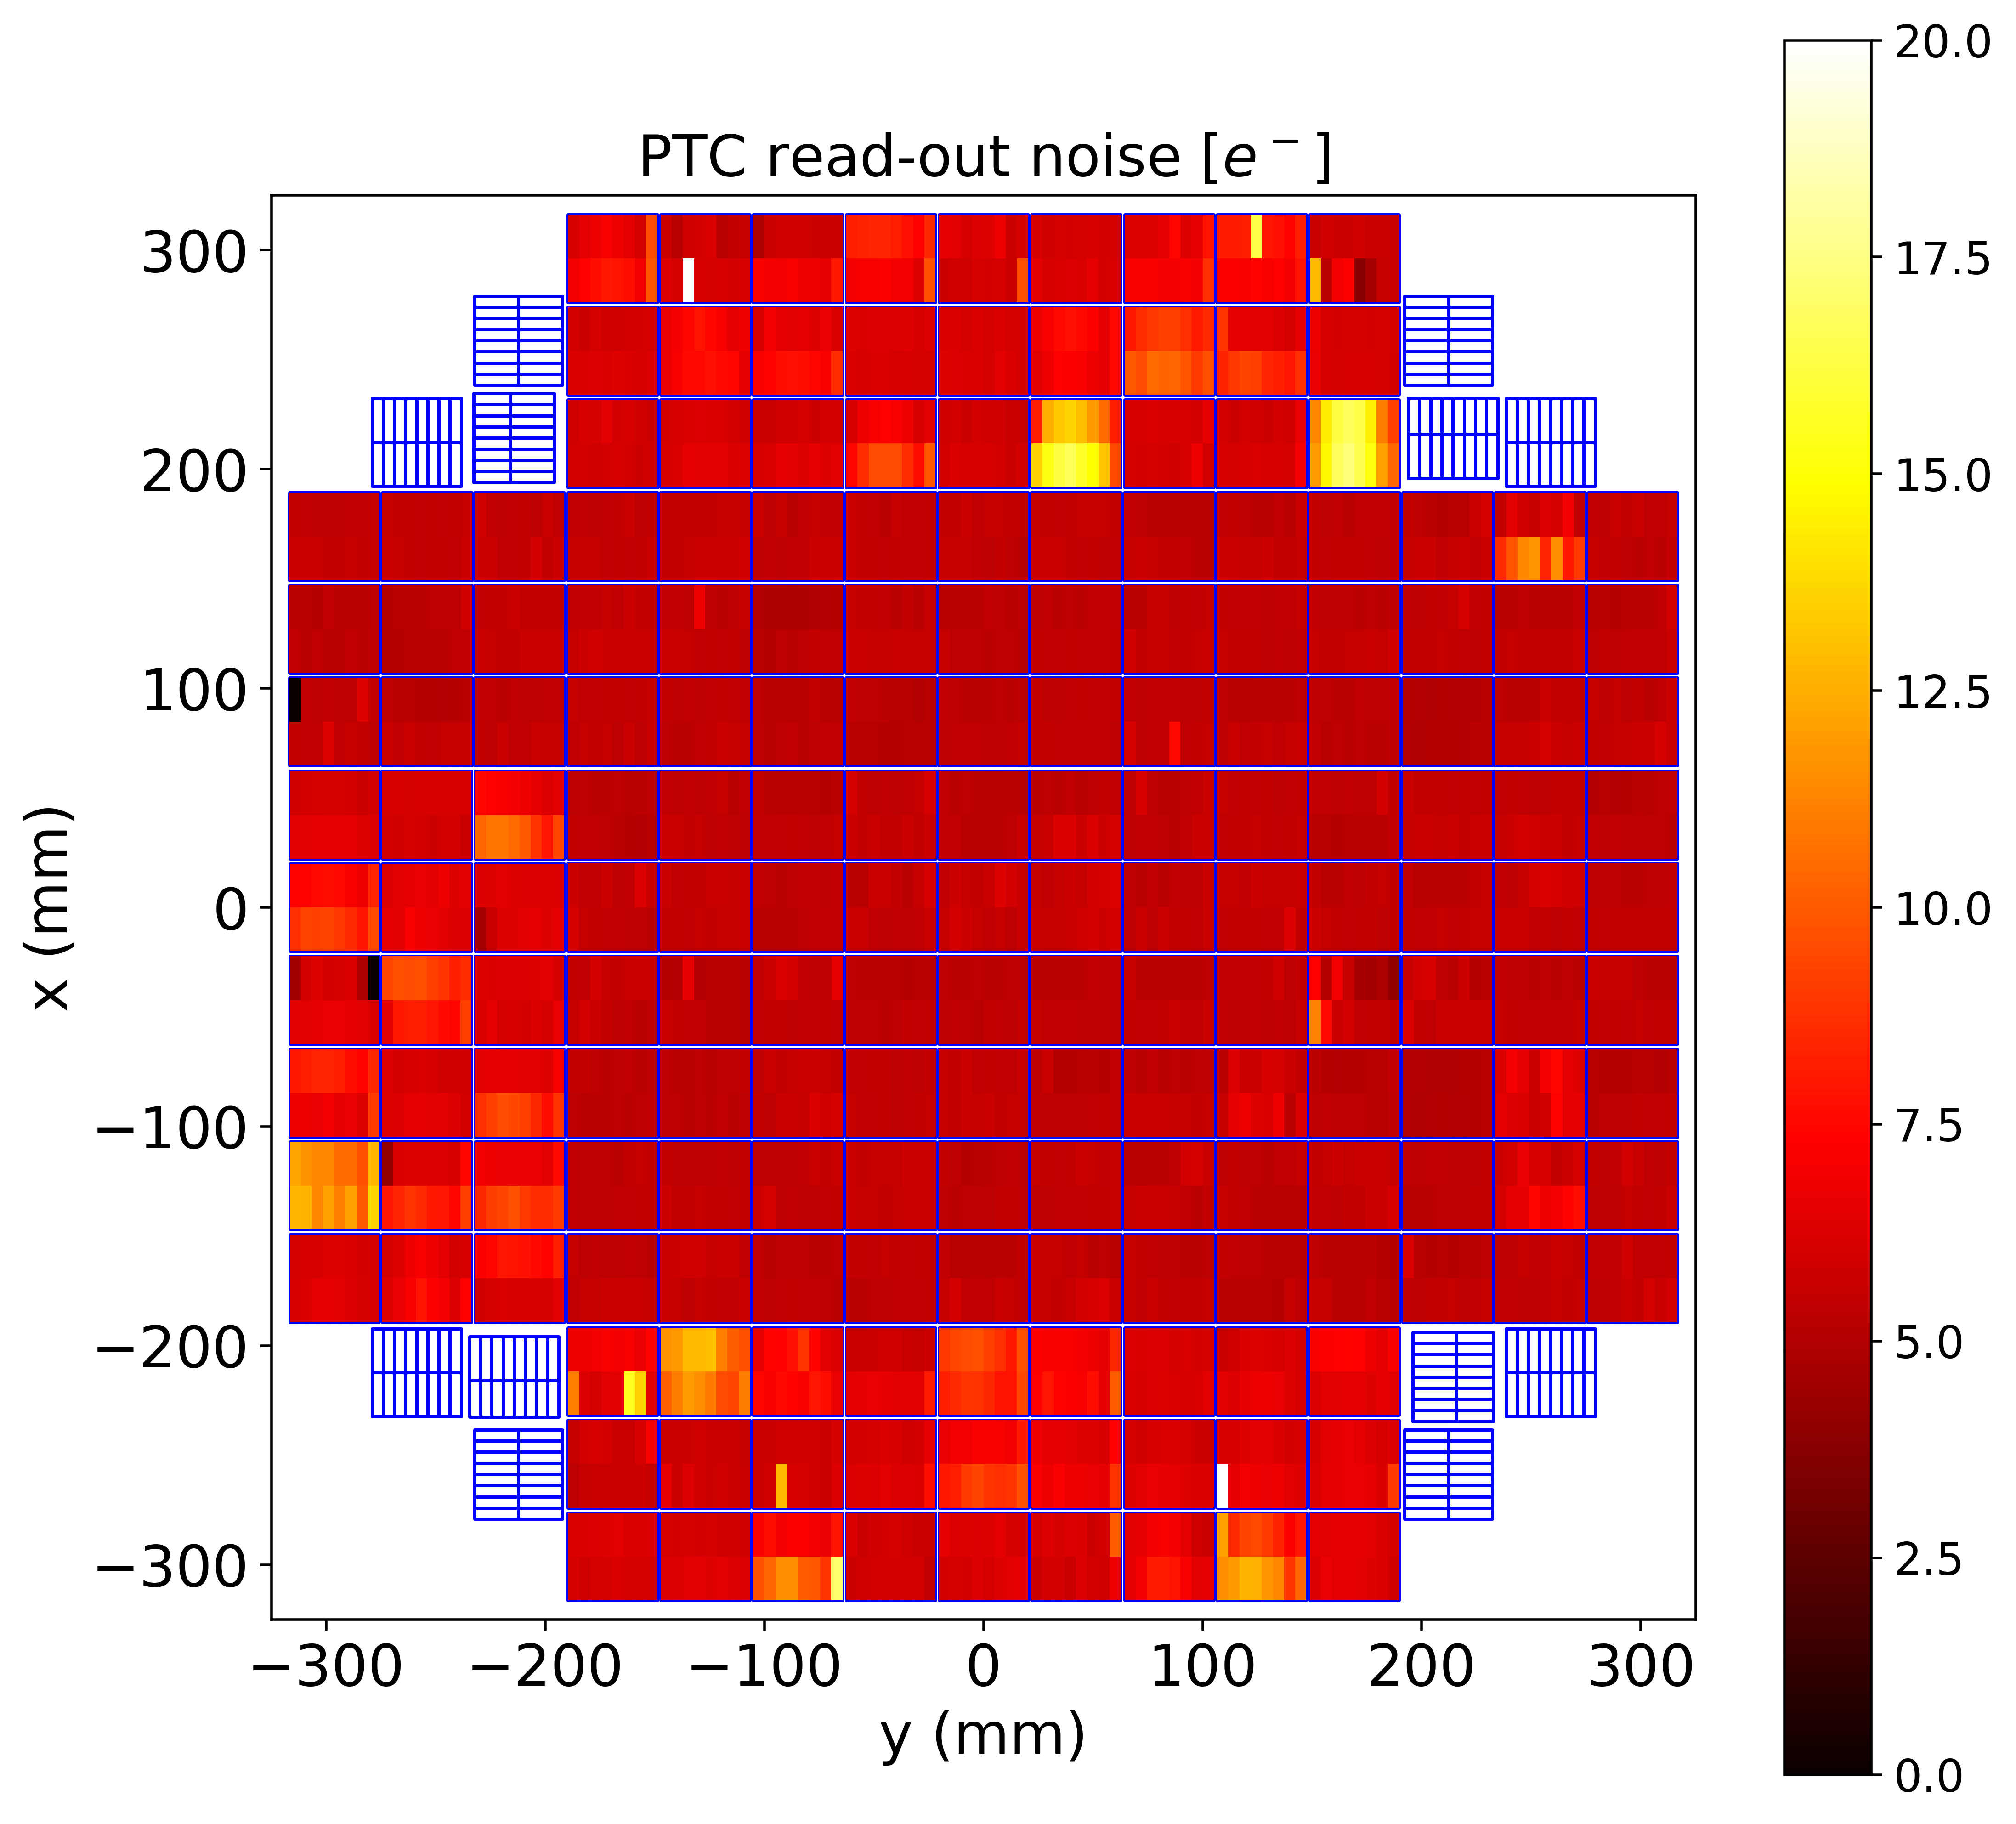
\includegraphics[width=\textwidth]{Figures/Focal_plane_noise.png}
     \end{subfigure}
     \vspace{3mm}
     \begin{subfigure}[b]{0.49\textwidth}
         \centering
         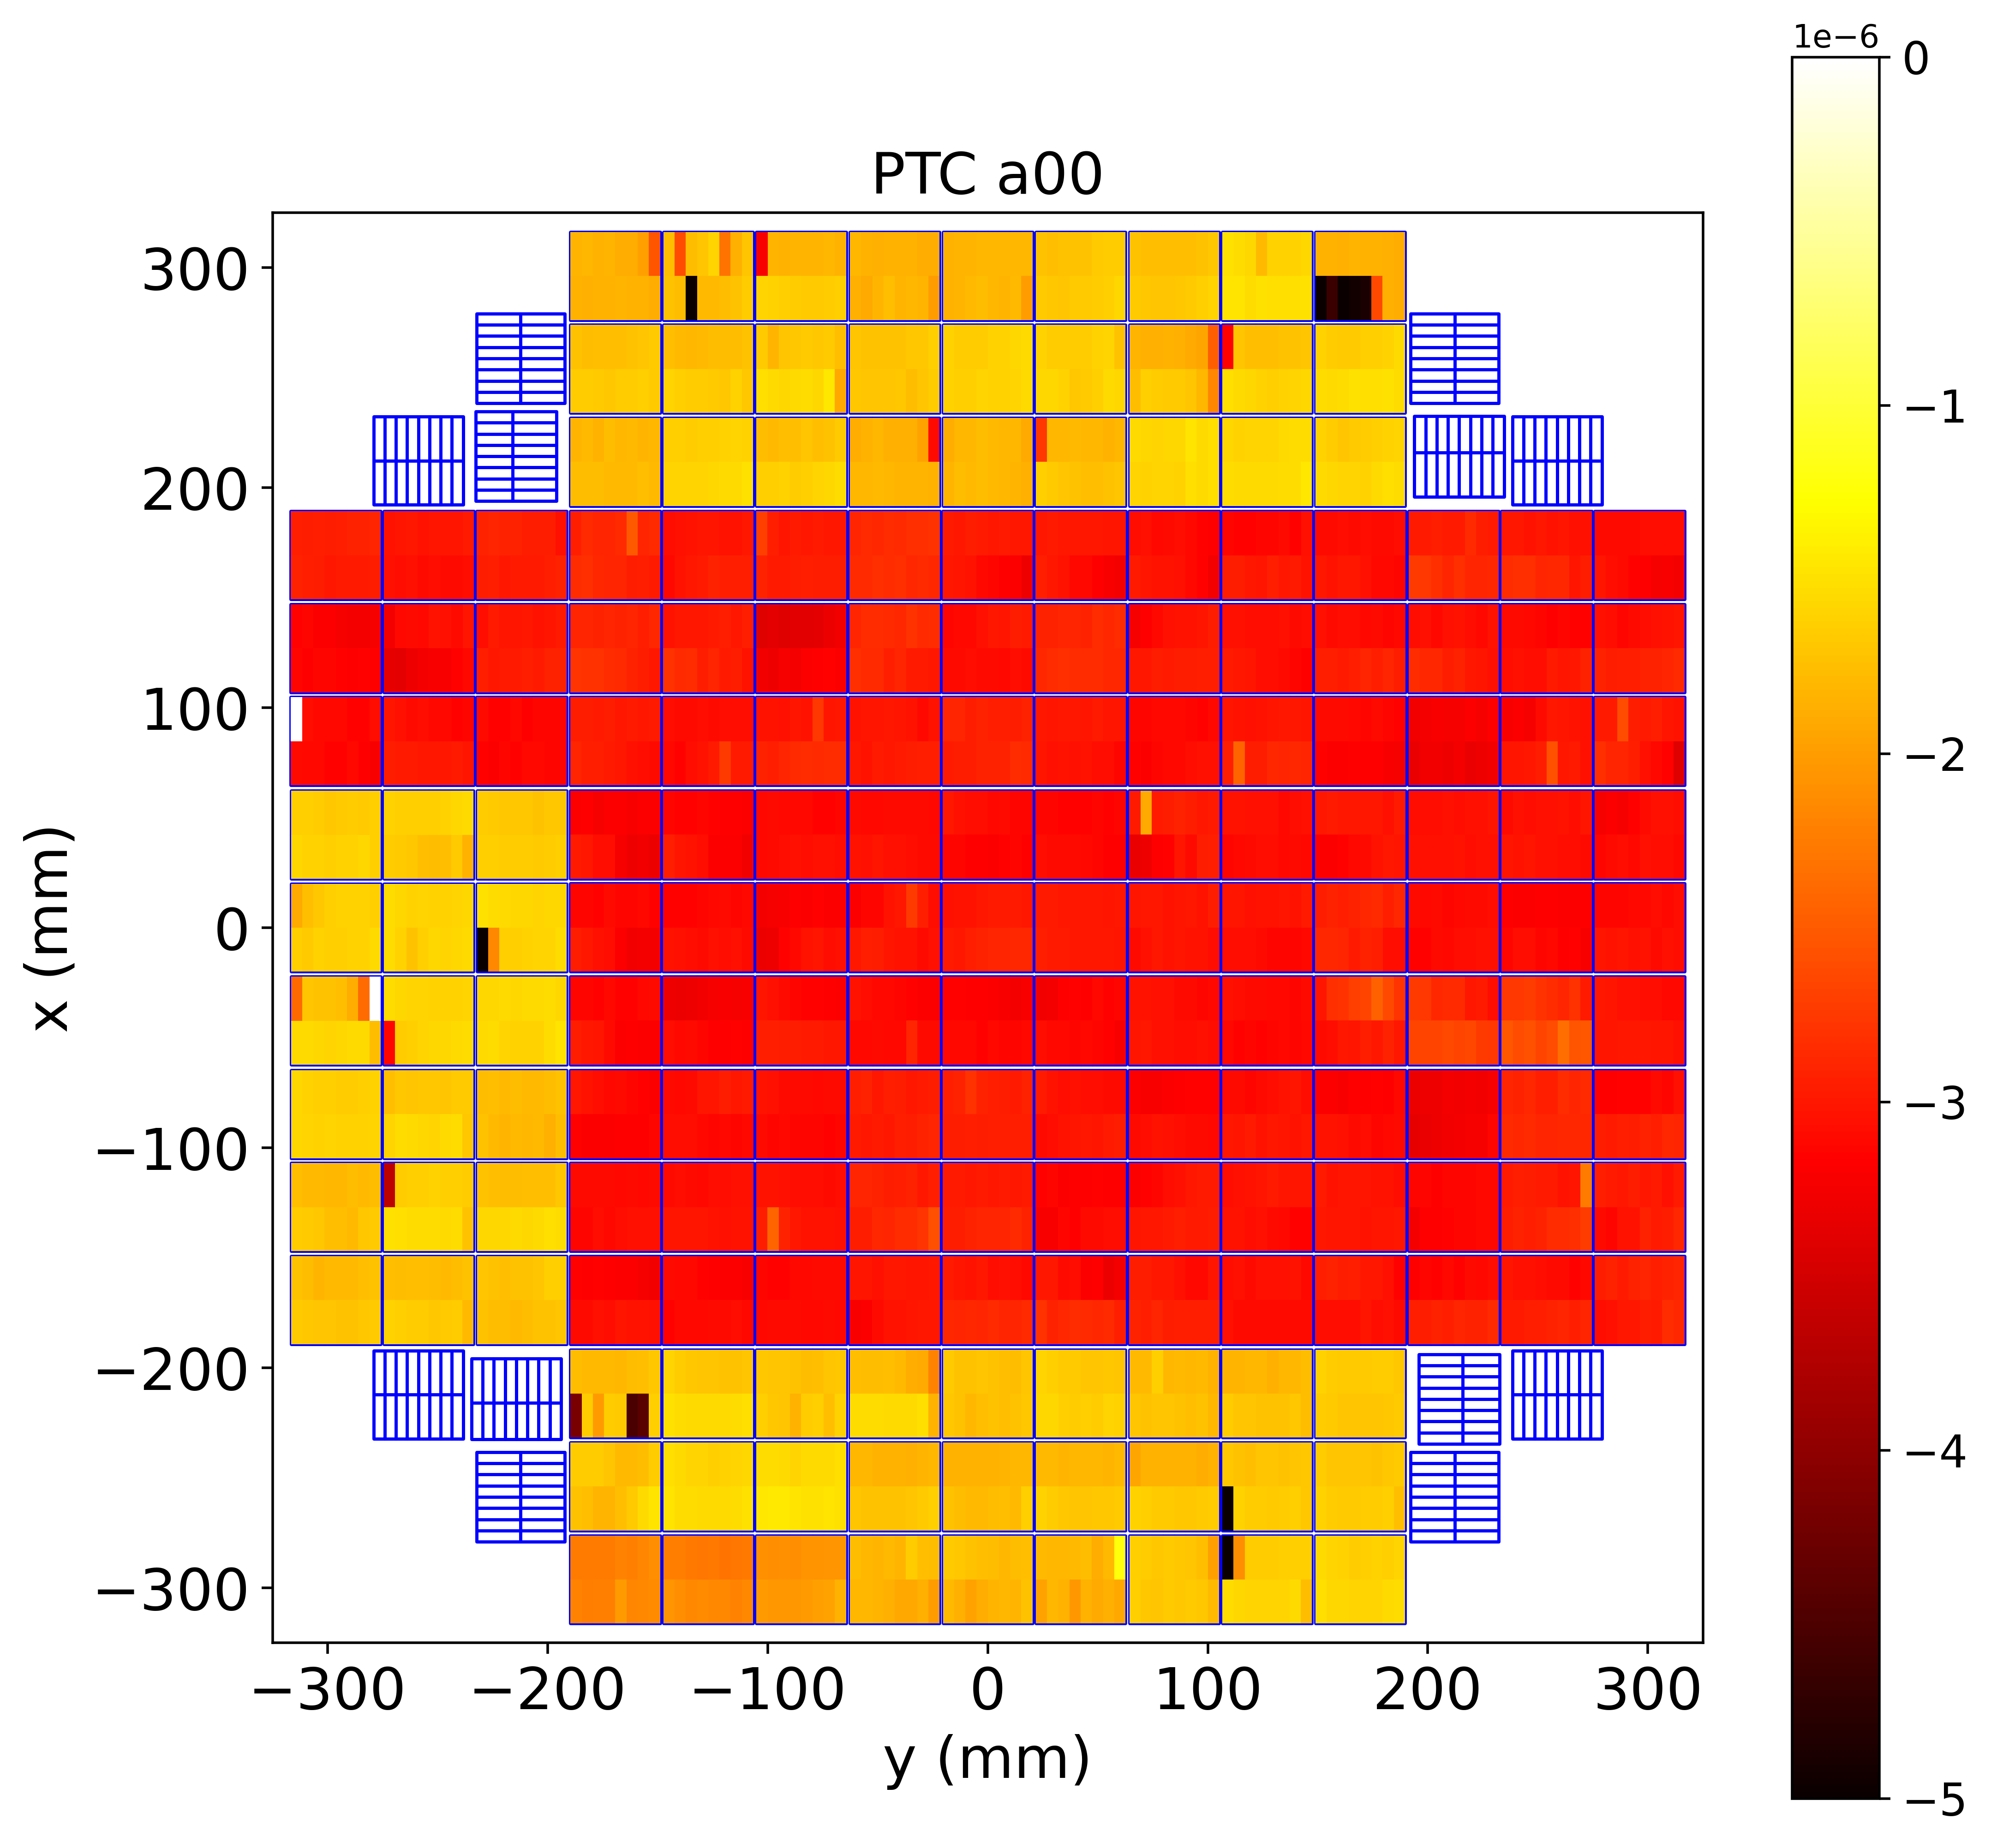
\includegraphics[width=\textwidth]{Figures/Focal_plane_a00.png}
     \end{subfigure}    
     \hfill
     \begin{subfigure}[b]{0.49\textwidth}
         \centering
         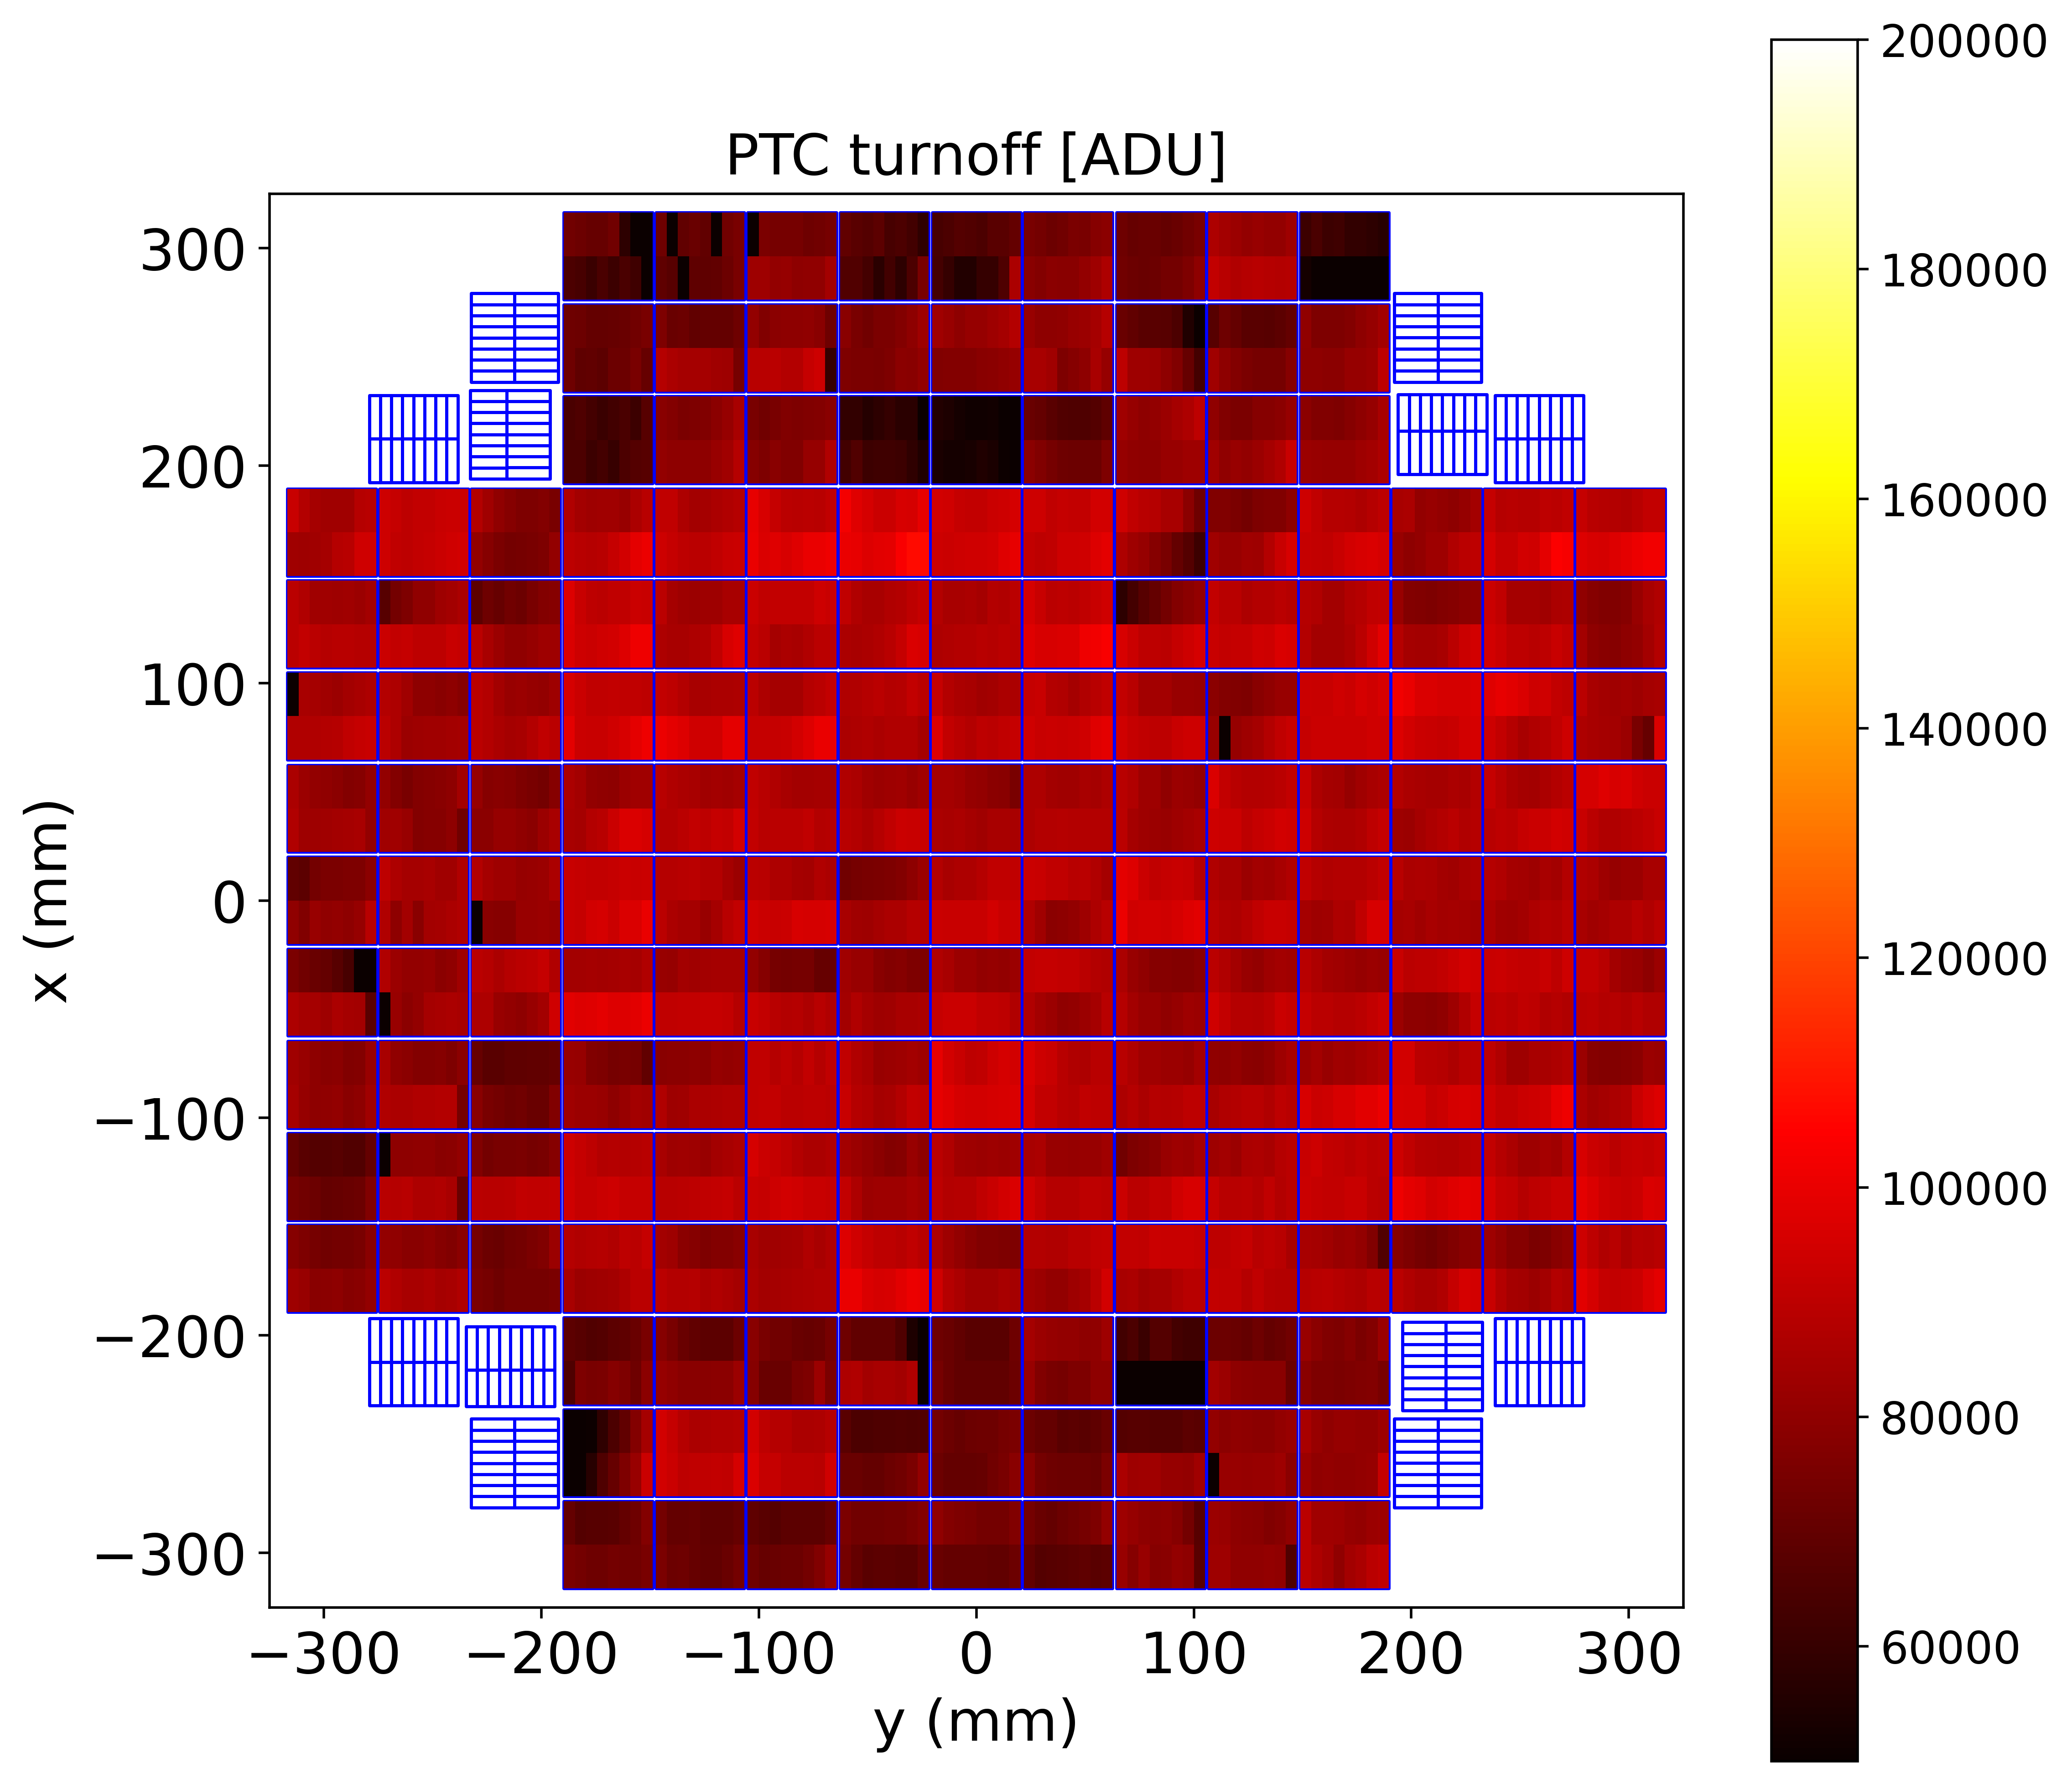
\includegraphics[width=\textwidth]{Figures/Focal_plane_turnoff.png}
     \end{subfigure}
        \caption{Heatmaps for the entire focal plane of the parameters obtained by the fit to the PTC in each segment that makes up the sensors. The upper panel shows the gain values on the left and the read noise on the right. The lower panel shows on the left the values of $a_{00}$, which are of the order of $-1 \times 10 ^{-6}$, and on the right, the turnoff. These maps are a reproduction of those already constructed by SLAC for this same run 13144 (\href{https://srs.slac.stanford.edu/BOT_EO_Reports/13144/}{SLAC heat maps}).}
        \label{fig:FocalPlane_PTC}
\end{figure}
%%%%%%%%%%%%%%%%%%

Subsequently, we generate heat maps for the entire focal plane similar to those performed by SLAC, shown in the panels of Figure \ref{fig:FocalPlane_PTC}, for the parameters estimated by the fit to the PTC: gain and read noise in the upper left and right panel, respectively; $a_{00}$ and turnoff in the lower left and right panel, respectively. A bimodality is found in the gain and $a_{00}$ value (which accounts for the B-F effect); the more reddish values dominate in the E2V sensors, while the more yellow values dominate in ITL; this means that the E2V vendor's detectors have in general a lower gain, but a more negative B-F effect coefficient concerning ITL. Whereas, for readout noise and turnoff, no relevant effect is exhibited due to the vendor. 

\vspace{3mm}

El comportamiento descrito anteriormente por los mapas de calor son reforzados por los histogramas de la figura \ref{fig:Histogram_PTC}, los cuales revelan la clara bimodalidad para la ganancia y $a_{00}$ y un comportamiento más generalizado para el ruido de lectura y el turnoff. La ganancia tiene un valor promedio para los sensores de E2V de $1.49 \pm 0.05$ y de $1.69 \pm 0.05$ $e^{-}/ADU$ para ITL. El coeficiente del B-F effect tiene un valor medio de $(-3.0 \pm 0.1)\times 10 ^{-6}$  y $(-1.7 \pm 0.2)\times 10 ^{-6}$ para E2V e ITL, respectivamente.

The histograms support the behavior described above by the heat maps in Figure \ref{fig:Histogram_PTC}, which reveal clear bimodality for gain and $a_{00}$ and more generalized behavior for read noise and turnoff. The gain has an average value for the E2V sensors of $1.49 \pm 0.05$ and $1.69 \pm 0.05$ $e^{-}/ADU$ for ITL. The BF effect coefficient has an average value of $(-3.0 \pm 0.1)\times 10 ^{-6}$ and $(-1.7 \pm 0.2)\times 10 ^{-6}$ for E2V and ITL, respectively.

\vspace{3mm}

%%%%%%%%%%%%Figura
\begin{figure}[!htb]
    \centering
    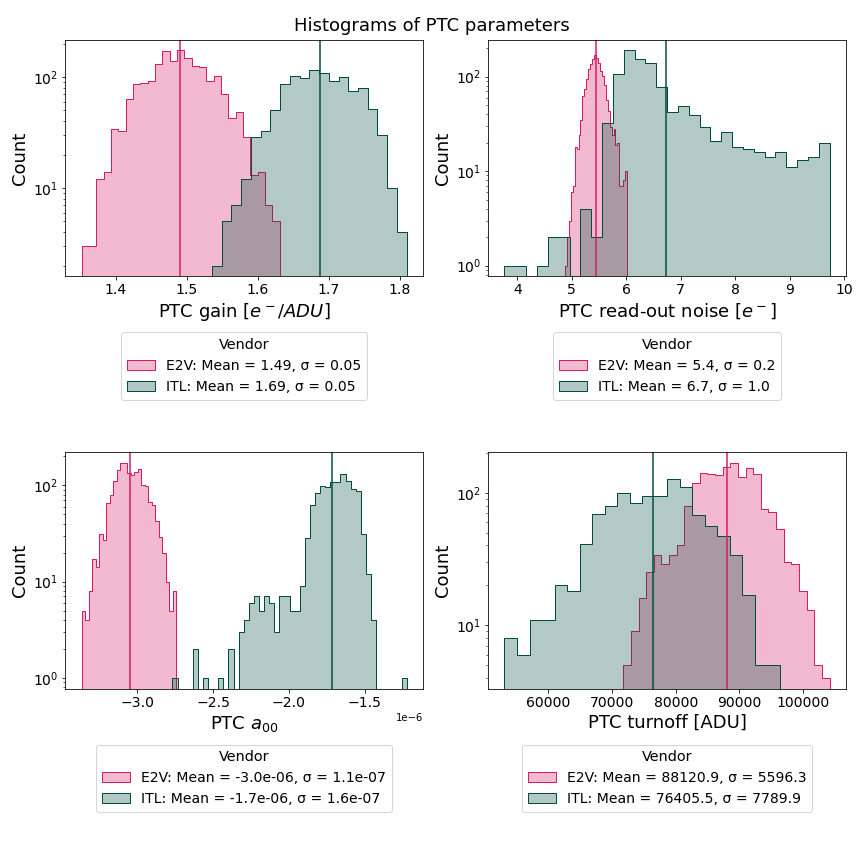
\includegraphics[width=\textwidth]{Figures/Histograms_PTC.png}
    \caption{Histograms for the parameters obtained from the fit to the PTC: gain (top left), read noise (top right), $a_{00}$ (bottom left), and turnoff (bottom right), each of the distributions are shown by vendor, in magenta for E2V and blue for ITL. The vertical lines represent the mean of each distribution. }
    \label{fig:Histogram_PTC}
\end{figure}

%%%%%%%%%%%%%%%%%%

Although, in general, the results between this work and SLAC are congruent, we find differences in some segments for gain, especially in segments C04 and C14 of detector 0 (R01\_S00), C00 of detector 22 (R03\_S11) and C02 of detector 169 (R41\_S21). In table \ref{tab:PTC_warnings} we report in red the segments where we found the most notorious difference between our and the SLAC results for the four parameters (gain, BF coefficient, read noise, and turnoff). For the segments mentioned above, the table shows that detector 22 is possibly dead; in contrast, for the segment of detector 169, there is a misclassification by the PTC-turnoff location algorithm. For these particular segments, the before mentioned can be the reason for the difference between SLAC and us. However, to determine which is causing the differences precisely, it is necessary to conduct a detailed analysis of the respective codes used and their versions. Differences between the algorithms may lead to these differences because we used the same run (13144). It can be differences in the pixels used for the calculation due to the masks used, differences in the reduction of the images (Instrument Signature Removal or ISR), or different rejection of outliers, among others. 


\vspace{3mm}

%%%%%%%%%%%%Figura

\begin{figure}[!htb]
%\raggedleft
     \begin{subfigure}[b]{\textwidth}
         
         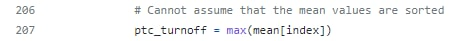
\includegraphics[width=0.7\textwidth,left]{Figures/eotest_turnoff.jpg}
         \caption{Eotest code}
     \end{subfigure}
     \vspace{3mm}
     \begin{subfigure}[b]{\textwidth}
         
         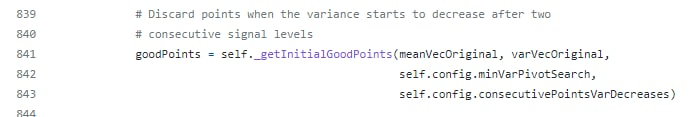
\includegraphics[width=\textwidth,left]{Figures/DMstack_turnoff1.jpg}
     \end{subfigure}    
     \vspace{3mm}
     \begin{subfigure}[b]{\textwidth}
         
         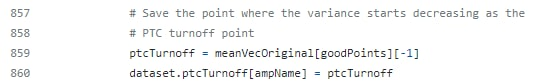
\includegraphics[width=0.85\textwidth,left]{Figures/DMstack_turnoff2.jpg}
         \caption{DM stack code}
     \end{subfigure}
        \caption{Codes used to calculate the PTC-turnoff in \href{https://github.com/lsst-camera-dh/eotest/blob/32c17b0a33b9c099651ed581ee90c1b1101012fb/python/lsst/eotest/sensor/ptcTask.py}{eotest}  (a), used by SLAC, and \href{https://github.com/lsst/cp_pipe/blob/6bae47012f2f119b186509ce7efd963b68b61f0d/python/lsst/cp/pipe/ptc/cpSolvePtcTask.py}{DM stack} (b), official code for LSST data.}
        %Códigos utilizados para calcular el PTC-turnoff en \href{https://github.com/lsst-camera-dh/eotest/blob/32c17b0a33b9c099651ed581ee90c1b1101012fb/python/lsst/eotest/sensor/ptcTask.py}{eotest} (a), empleado por SLAC, y \href{https://github.com/lsst/cp_pipe/blob/6bae47012f2f119b186509ce7efd963b68b61f0d/python/lsst/cp/pipe/ptc/cpSolvePtcTask.py}{DM stack} (b), código oficial para los datos del LSST.}
        \label{fig:Turnoff_codes}
\end{figure}
%%%%%%%%%%%%%%%%%%


For the turn-off, we generally observed similar behavior for the sensors between this work and SLAC. However, the way of determination used different methods, as shown in figure \ref{fig:Turnoff_codes}. On the one hand, \textit{eotest} defines the PTC-turnoff as the point where the variance is maximum, where the maximum value is determined among the data whose residuals are below $5sigma$. In contrast, \textit{DM stack} defines this as the point where the variance starts to decrease monotonically by at least two points (the number of points to decrease can be modified in the function \_getInitialGoodPoints). By SLAC, the FWC found was $\sim 90000$ e$^-$ \colorbox{red}{referencia?}. In contrast, in this work, we found an average value of turnoff with a value of $83240$ ADU, whose equivalence in electrons would be an approximate value of the FWC of $130000 \pm 10000$ e$^-$.

\begin{landscape}
\begin{table}[!htb]
\centering
\caption{Detectors containing segments with low PTC-turnoff (below 40000 ADU), PTC-turnoff misclassified by the algorithm, bad segments, or differences observed concerning the results obtained by SLAC (parameters in red). Presented for each segment is the detector ID (col1), detector number (col2), vendor (col3), affected segment (col4), PTC parameters (gain, B-F effect, and turnoff coefficient; cols 5, 6, 7, and 8, respectively), detected problem (col9).}
\label{tab:PTC_warnings}
\begin{tabular}{ccccccccp{0.2\textwidth}}
    \hline 
     Detector ID   &   Det Num & Vendor   & Amp   &     Gain &   Read Noise &           $A_{00}$ &   Turnoff & Issue\\
      & & & & $[e^-/$ADU$]$ & $[e^-]$ & & [ADU] & \\
    \hline 
    \hline
    R01\_S00       &              0 & ITL      & C04  &   \textcolor{red}{1.5833} &   6.2061                 &  $\textcolor{red}{-2.0160 \times 10^{-6}}$ & 73461.2   &  SLAC diff \\
    R01\_S00       &              0 & ITL      & C14  &   \textcolor{red}{1.7514} &   6.4150                 &  $\textcolor{red}{-2.1907 \times 10^{-6}}$ & 68032.3   &  SLAC diff \\
    R01\_S20       &              6 & ITL      & C00  &   \textcolor{red}{1.5354} & \textcolor{red}{11.1174} &  $\textcolor{red}{-4.1734 \times 10^{-6}}$ & 65371.7   &  SLAC diff \\
    R01\_S20       &              6 & ITL      & C05  &   \textcolor{red}{1.4837} & \textcolor{red}{15.5104} &  $\textcolor{red}{-4.5175 \times 10^{-6}}$ & 76106.5   &  SLAC diff \\
    R01\_S20       &              6 & ITL      & C06  &   \textcolor{red}{1.5104} & \textcolor{red}{13.5644} &  $\textcolor{red}{-4.3955 \times 10^{-6}}$ & 72293.9   &  SLAC diff \\
    R02\_S20       &             15 & ITL      & C17  &      1.67191              &      5.81973             &  $-2.20396 \times 10^{-6}$                 & 30567.4   & low PTC-turnoff\\
    R03\_S11       &             22 & ITL      & C00  & \textcolor{red}{15.2117}  & \textcolor{red}{44.0087} &  \textcolor{red}{-0.708105}                & 223.072   & SLAC diff - dead?\\
    R10\_S11       &             31 & ITL      & C10  &      1.63413              &      4.13177             &  $-3.65785 \times 10^{-6}$                 & 32842.4   & low PTC-turnoff\\
    R20\_S00       &             72 & ITL      & C17  &      0                    &  \textcolor{red}{0}      & nan                                        &     0     & SLAC diff and dead\\
    R20\_S01       &             73 & ITL      & C00  &      1.6083               &      6.45279             &  $-3.12539 \times 10^{-6}$                 & 35507.4   & low PTC-turnoff\\
    R20\_S12       &             77 & ITL      & C00  &      1.59232              &      4.70427             &  $-8.02249 \times 10^{-6}$                 & 26827.1   & low PTC-turnoff\\
    R30\_S00       &            117 & E2V      & C10  &      0                    &  \textcolor{red}{0}      & nan                                        & 0         & SLAC diff and dead\\
    R41\_S20       &            168 & ITL      & C16  &      1.61074              &      6.07818             &  $-1.98753 \times 10^{-6}$                 & 37863.2   & low PTC-turnoff\\
    R41\_S20       &            168 & ITL      & C17  &      1.59228              &      9.57256             &  $-2.54637 \times 10^{-6}$                 & 26120     & low PTC-turnoff\\
    R41\_S21       &            169 & ITL      & C02  & \textcolor{red}{1.08095}  & \textcolor{red}{62.8775} &  $-4.52943 \times 10^{-6}$                 & 16237.9   & SLAC diff and PTC-turnoff mismatch\\
    R41\_S21       &            169 & ITL      & C11  &      1.61255              &      5.23312             &  $-2.61051 \times 10^{-6}$                 & 32467.3   & PTC-turnoff mismatch\\
    R41\_S21       &            169 & ITL      & C15  &      1.59804              &      5.21757             &  $-2.31531 \times 10^{-6}$                 & 39151.3   & PTC-turnoff mismatch\\
    R41\_S22       &            170 & ITL      & C10  &      1.60171              &      4.76741             &  $-3.2105  \times 10^{-6}$                 & 32369.9   & low PTC-turnoff\\
    R42\_S00       &            171 & ITL      & C17  &      1.6516               &      6.4254              &  $-3.09362 \times 10^{-6}$                 & 30253.3   & low PTC-turnoff\\
    R43\_S10       &            183 & ITL      & C17  &      1.59721              &      8.53352             &  $-2.46596 \times 10^{-6}$                 & 30195.2   & low PTC-turnoff\\
    R43\_S22       &            188 & ITL      & C00  &      1.6348               & \textcolor{red}{5.28826} &  $-4.64678 \times 10^{-6}$                 & 21477.5   & SLAC diff\\
    R43\_S22       &            188 & ITL      & C01  &      1.6348               &      5.28826             &  $-4.64678 \times 10^{-6}$                 & 21477.5   & low PTC-turnoff\\
    R43\_S22       &            188 & ITL      & C02  &      1.55382              &      6.94625             &  $-7.40255 \times 10^{-6}$                 & 30764.3   & low PTC-turnoff\\
    R43\_S22       &            188 & ITL      & C03  &      1.56826              &      7.24918             &  $-4.92713 \times 10^{-6}$                 & 38222.4   & low PTC-turnoff\\
    R43\_S22       &            188 & ITL      & C04  &      1.58147              &      3.76291             &  $-4.88158 \times 10^{-6}$                 & 38143.6   & low PTC-turnoff\\
    \hline
    \end{tabular}
\end{table}
\end{landscape}

\subsection{Gain from flat pairs}

Initially, we used the PTC to obtain the gain. However, this method requires more time to be generated since it is a fit over an extensive range in flow. Therefore, we have an alternative approach, which we will call \textit{gain by pairs of flats}, less time-consuming. The left panel of the figure \ref{fig:Gain_full} shows for detector 55 the gain values in a range of flux between $0$ to $\sim 120000$ ADU, which includes values that have exceeded the saturation level given by the vertical lines marking the PTC-turnoff for each segment. On the right panel, the gain values are only a little further away from the saturation level, and we can see a bump around 60000 ADU due to the nonlinearity, which will be discussed in section \ref{subsec:crosstalk_and_linearity}. It is worth mentioning that we only use data below the PTC-turnoff for the analysis of the gain per pair of flats. 
 
\vspace{3mm}
In this section, we describe the differences we found between the gain by PTC and pairs of flats, a possible way to decrease them, and finally, what to expect from this second method concerning the first one.

 \begin{figure}[!htb]
    \centering
    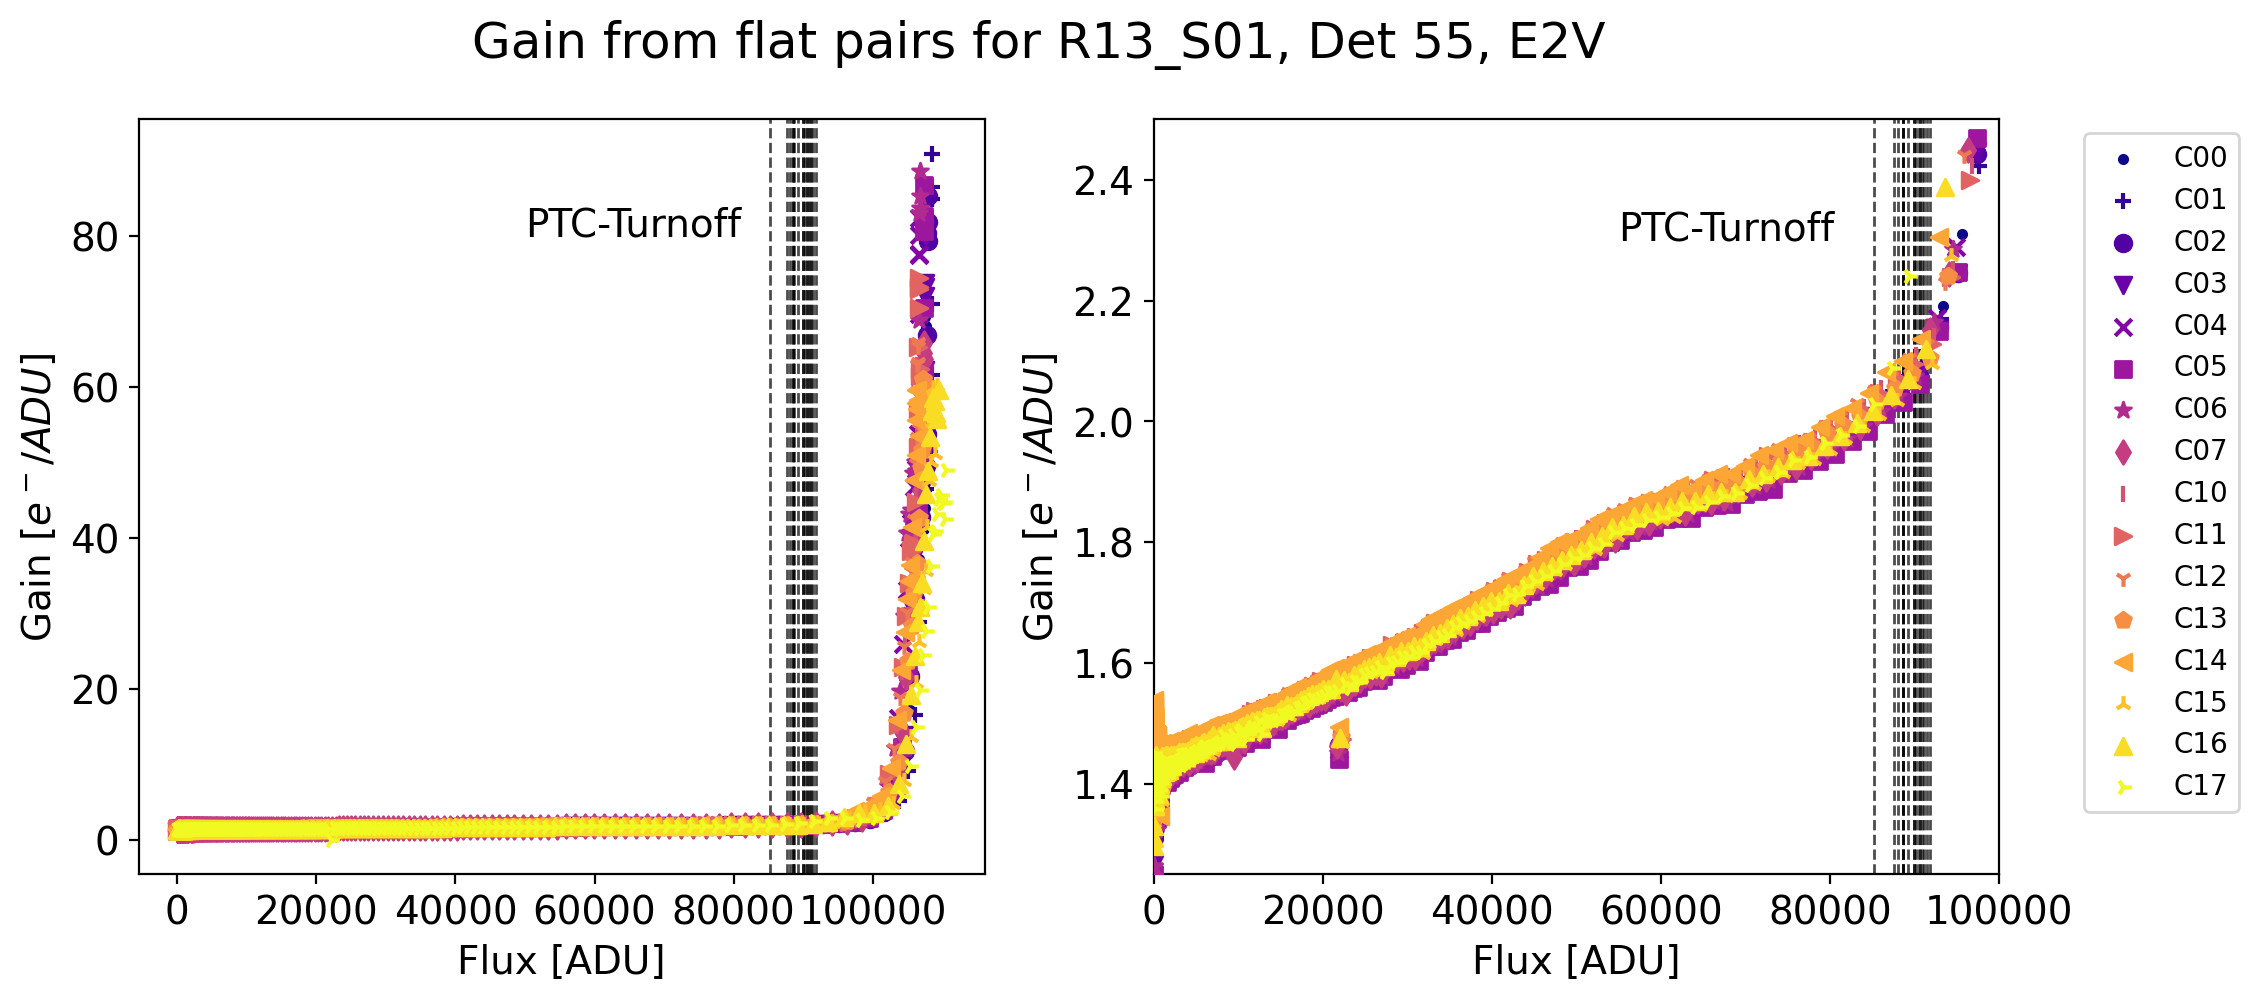
\includegraphics[width=\textwidth]{Figures/Gain_plot_55.png}
    \caption{Gain values obtained by flat pairs for fluxes up to approximately 120000 ADU for detector 55 (R13\_S01). In both panels, the dashed vertical lines represent the PTC turnoff value for each of the 16 detector segments, and the colored figures represent the gain and flux values for each segment. The right panel shows only the region up to the PTC-turnoff of the left panel.}
    \label{fig:Gain_full}
\end{figure}

\vspace{3mm}

As we mentioned in the methodology (sec. \ref{sec:methods}), we used two code versions (w\_2022\_27 and w\_2022\_32), where the main difference and our interests is the one shown in figure \ref{fig:diff_codes}. This figure shows how the two code versions handled the statistics to compute gain by pairs of flats. The \textit{w\_202222\_27} version used the red code with the assumption of a Gaussian distribution, so it truncates the distribution to reject outliers. Whereas the \textit{w\_2022\_32} version used the green code rejecting the before assumption. The last one is our recommendation due to the analysis results described in this section. In short: the distribution of the operation between two flats images leading to calculating the gain does not have a Gaussian distribution, so performing a truncation in the distribution alters the expected value for the gain.


\begin{figure}[!htb]
    \centering
    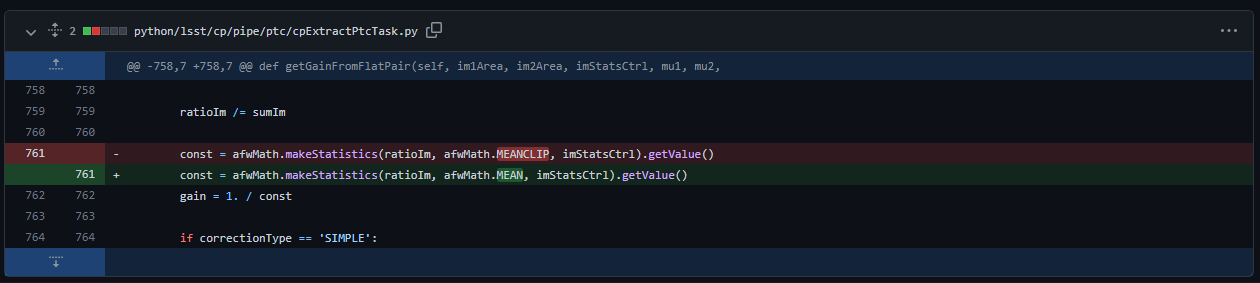
\includegraphics[width=\textwidth]{Figures/Cambio_codigo.png}
    \caption{Difference between the initial(w\_2022\_27, in red) and current (w\_2022\_32, in green) codes for calculating the gain from a pair of flat fields.}
    \label{fig:diff_codes}
\end{figure}

The version \textit{w2022} gave us the result shown in figure \ref{fig:relative_error_oldcode}, a relative percentage error between the gain per PTC and flat pair at a flux of 5000 ADU above 5 \%, the same result for an E2V detector (upper panel) and an ITL detector (lower panel). This high percentage at this flux was not expected, so we performed simulations with the methodology described in section \ref{subsubsec:method_Simulation_Gain} to investigate what was generating this value.


\subsubsection{Simulation}

From the previous result, a relative error between the gains of 5 \% at 5000 ADU, we had some hypotheses: first, the masks in the flat images could be affecting in some way, e.g.,  if the masks of each image are very different and the code uses these to make calculations, it could generate a high relative error; second, an overestimation in the read noise; and third, if it is not the masks, so what in the statistics is causing this error. 

\vspace{3mm}

We found from simulations of a flat image of a CCD segment and using the mask of an actual segment: the use of one mask for the two flats, the union of both masks, or different masks for each do not account for the error of 5 \% at 5000 ADU, as shown in the top panel of Figure \ref{fig:simulation_masks}. We notice in this case that the higher the read noise, when using a NONE type correction, the more significant the discrepancies between the expected and calculated gain (2 $e^-$/ADU). However,  the subsequent corrections (SIMPLE and FULL), which account for the read noise, accurately calculate the expected gain value. Nonetheless,  the bottom panel of this figure, which includes, besides the masks, the control statistics, gives an account in all cases of a relative percentage error between the gain per PTC and flats pairs above 5 \%. In the next section (\ref{subsubsec:results_gainflats_realdata}) we check this with the real data.

%Encontramos a partir de las simulaciones de la imagen flat de un segmento de CCD, utilizando una máscara de un segmento real, que utilizar una máscara para los dos flats, la unión de ambas máscaras o máscaras diferentes para cada uno, no daba cuenta del error del 5\% a 5000 ADU, tal y como lo muestra el panel superior de la figura \ref{fig:simulation_masks},lo único que podemos ver en este caso es que a mayor ruido de lectura, y al utilizar una corrección de tipo NONE, mayores son las discrepancias entre la ganancia esperada (2 $e^-$/ADU) y la calculada, pero las subsecuentes correcciones (SIMPLE y FULL) que sí tienen en cuenta el valor del ruido de lectura logran calcular de forma precisa el valor esperado de ganancia. No obstante, el panel inferior de esta figura, que incluye además de las máscaras estadísticos de control, me da cuenta en todos los casos de un error relativo porcentual entre la ganancia por PTC y pares de flats por encima del 5 \%. En la siguiente sección (\ref{subsubsec:results_gainflats_realdata}) comprobamos esto con los datos reales.



\begin{figure}[!htb]
     \centering
     \begin{subfigure}[b]{\textwidth}
         \centering
         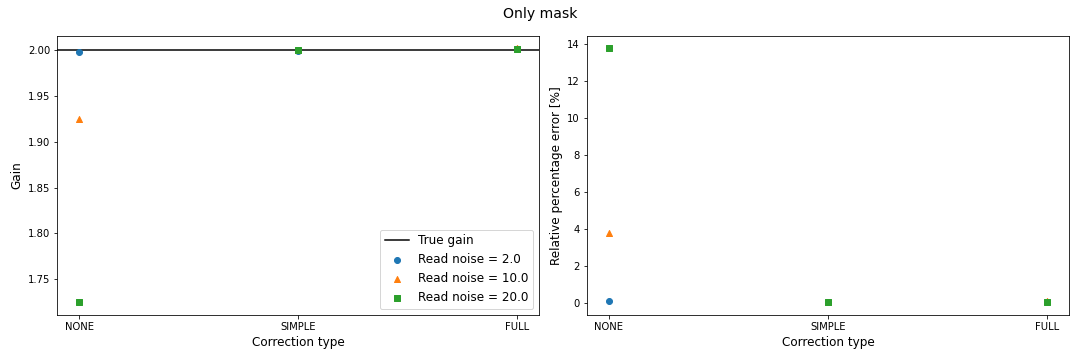
\includegraphics[width=\textwidth]{Figures/Simulation_masks.png}
     \end{subfigure}
     \vspace{3mm}
     \begin{subfigure}[b]{\textwidth}
         \centering
         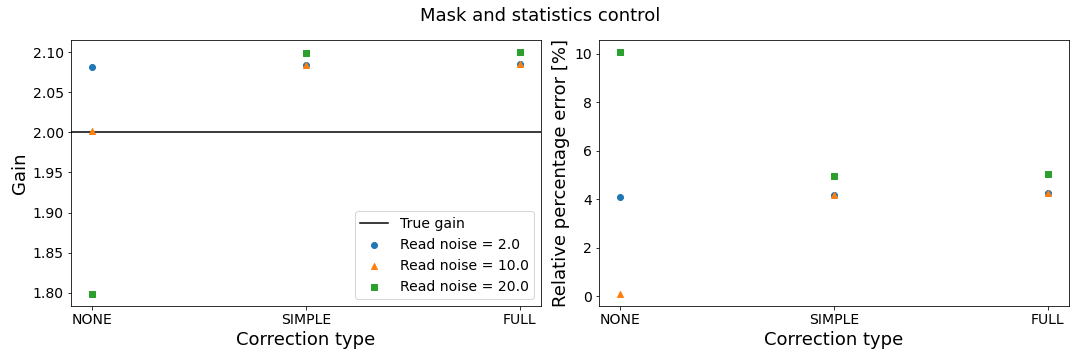
\includegraphics[width=\textwidth]{Figures/Simulation_masks_stats.png}
     \end{subfigure}
        \caption{Simulation results to obtain the gain per pair of flats in the upper panel using only masks and in the lower panel adding control statistics. The average flux value of these simulated flats is $5000$. The left panels show the gain value for three different models, and on the right, the relative percent error concerning the expected gain value, 2 $e^-/$ADU. In the left panels, the horizontal black line represents the predicted gain value, and the figures represent the different values considered for the read noise: the blue circle of 2 $e^-$, the orange triangle of 10 $e^-$, and the green square of 20$e^-$. Considering these read noises, we calculated the gain for three models: NONE, SIMPLE and FULL.}
        %Resultados de la simulación para obtener la ganancia por pares de flats, en el panel superior utilizando únicamente máscaras y en el inferior añadiendo además estadísticos de control. El valor promedio de flujo de estos flats simulados es de $\sim 5000$. Los paneles de la izquierda muestran el valor de la ganancia para 3 diferentes modelos y a la derecha el error relativo porcentual respecto al valor esperado de ganancia, 2 $e^-/$ADU. En los paneles izquierdos la línea negra horizontal representa el valor de ganancia esperado y las figuras representan los diferentes valores considerados para el ruido de lectura: círculo azul de 2 $e^-/$, triángulo naranja de 10 $e^-/$ y cuadrado verde de 20$e^-/$. Considerando estos ruidos de lectura se calculó la ganancia para tres modelos diferentes: NONE, SIMPLE y FULL.}
        \label{fig:simulation_masks}
\end{figure}

\subsubsection{Real data} \label{subsubsec:results_gainflats_realdata}
 
 Because of the results obtained from the simulation, we checked whether the results held with the actual data, and indeed they did. We performed this check on detector 55 (R13\_S01) for all its segments, as shown in figures \ref{fig:GainFlats_NOstats} and \ref{fig:GainFlats_stats}, where the black crosses represent the gain value obtained from the PTC. The first figure again reveals that the masks and no control statistics do not account for a relative error more significant than 5 \% for any segment of the detector; indeed, the maximum value achieved is 2.25 \% at an average flux of 5450 ADU. In the before result, we used the same mask for calculations: the union of the individual masks. The second figure, which uses the masks and incorporates the control statistics, shows that the handling of the statistics is producing high discrepancies between the gain by PTC and pairs of flats, reaching differences of up to 9 \% in one of the segments at a flow rate of 5450 ADU.
 
%En vista de los resultados obtenidos a partir de la simulación, se verificó si los resultados se mantienen con los datos reales y en efecto lo hacen. Hicimos esta comprobación en el detector 55 (R13\_S01) para todos sus segmentos, como se muestra en las figuras \ref{fig:GainFlats_NOstats} y \ref{fig:GainFlats_stats}, donde las cruces negras representan el valor de ganancia obtenida a partir de la PTC. La primera figura nuevamente revela que el uso de las máscaras (misma máscara utilizada para los cálculos, que es la unión de las máscaras individuales) y sin estadísticos de control no da cuenta de un error relativo mayor al 5 \% para ningún segmento del detector, el máximo valor alcanzado es de 2.25 \% a un flujo promedio de 5450 ADU. La segunda figura, que incorpora además los estadísticos de control, en cambio muestra que, en efecto, el manejo de los estadísticos está produciendo altas discrepancias entre la ganancia por PTC y la ganancia calculada por pares de flats llegando a alcanzar diferencias hasta del 9 \% en uno de los segmentos a un flujo de 5450 ADU.
 
\begin{figure}[!htb]
    \centering
    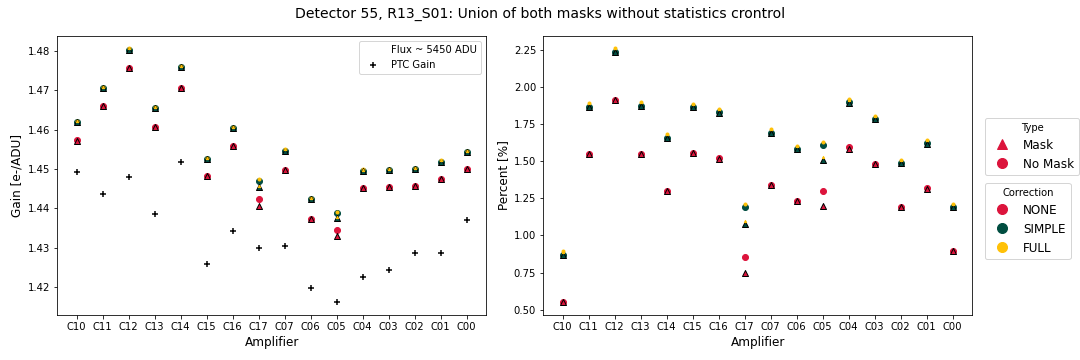
\includegraphics[width=\textwidth]{Figures/GainFlats_NOstats_det55.png}
    \caption{Gain value on the left panel and the relative percentage error on the right panel for the 16 segments (amplifiers) of detector 55 (R13\_S01). In the left panel, the black crosses represent the value of the gain per PTC. For both panels, the figures represent whether the calculation of the gain from flat pairs used mask (triangles) or not (circles) and the colors are associated with the model used to determine the gain: NONE (red), SIMPLE (green) and FULL (yellow). The mask for calculation was the union of the masks of both flat images per segment, and we did not use control statistics.}
    %Valor de ganancia (panel izquierdo) y error relativo porcentual (panel derecho) para los 16 segmentos (amplifier) del detector 55 (R13\_S01). En el panel izquierdo las cruces negras representan el valor de la ganancia por PTC. Para ambos paneles las figuras representan si el cálculo de la ganancia por pares de flats utilizó máscara (triángulos) o si no la utilizó (círculos), y los colores están asociados al modelo empleado para determinar la ganancia: NONE, SIMPLE y FULL. Para la máscara se utilizó la unión de las máscaras de ambas imágenes flat por segmento y no se utilizó estadísticos de control.}
    \label{fig:GainFlats_NOstats}
\end{figure}

\begin{figure}[H]
    \centering
    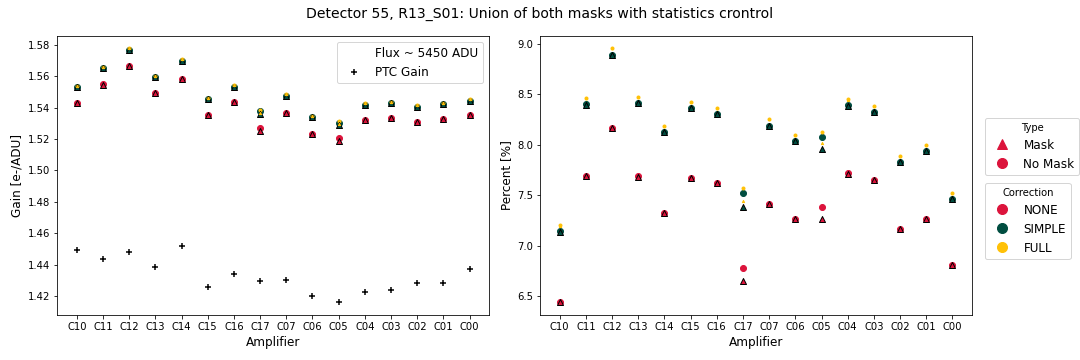
\includegraphics[width=\textwidth]{Figures/GainFlats_stats_det55.png}
    \caption{See description of the figure \ref{fig:GainFlats_NOstats}. This figure used control statistics.}
    \label{fig:GainFlats_stats}
\end{figure}
 
 
Subsequently, we performed plots of the distributions for the operation between the flats images given by the equation \ref{eq:ratioIm}, which is the argument of the Lupton equation (eq. \ref{eq:Lupton}) and is directly related to the gain. The results we obtained are shown in figure \ref{fig:hist_ratioIM} for each detector segment and reveal that the shape of this distribution is far from Gaussian. So truncating this distribution produces a change in the mean value, which no longer coincides with the mean of the original distribution, thus giving a different gain value than expected. 

\vspace{3mm}

Finally, we again constructed the relative percentage error figures for the gain without truncating the distribution, as shown by the green code in figure \ref{fig:diff_codes}. We obtained the result in figure \ref{fig:relative_error}, which reveals in its embedded image that for a flow of 5000 ADU, the difference between the two gains is now below 5 \%, as indicated by the simulations. With this result, we estimate a general relationship for the gain taking into account the distributions for the linear fit parameters, as shown in figure \ref{fig:histogram_linearfit}, which was performed between 5000 and 10000 ADU. In this figure, we can see on the top left the distribution of the slopes by the vendor, which reveals a clear bimodality, with the E2V detectors having a slightly higher slope concerning ITL, with a mean of $(0.00046 \pm 0.00004)$ and $(0.00027 \pm 0.00004)$ \%/ADU, respectively. In the bottom panel of this figure, we have the intercept with the y-axis (i.e., with the percentage error axis between the gains), and it shows that there is an overall mean across the detectors, with no appreciable distinction by vendor, with a value of $(-0.5 \pm 0.5)$ \%. Thus, by vendor, the relative percentage error between the 5000 and 1000 ADU is given by


%Finalmente, sin efectuar truncamiento en la distribución, como lo muestra el código en verde de la figura \ref{fig:diff_codes}, construimos nuevamente las figuras de error relativo porcentual para la ganancia y obtuvimos el resultado de la figura \ref{fig:relative_error} que revela en su imagen embebida que para un flujo de 5000 ADU que la diferencia entre ambas ganancias ahora está por debajo del 5 \% como lo indicaban las simulaciones. Con este resultado estimamos una relación general para la ganancia teniendo en cuntra las distribuciones para los parámetros del ajuste lineal, como se muestran en la figura \ref{fig:histogram_linearfit}, que fue efectuado entre los 5000 y 10000 ADU. En esta figura se observa a la izquierda arriba la distribución de las pendiente por fabricante que revela una clara bimodalidad, teniendo una pendiente ligeramente mayor los detectores de E2V respecto a ITL, con una media de $(0.00046 \pm 0.00004)$ y $(0.00027 \pm 0.00004)$ \%/ADU, respectivamente. En el panel inferior de esta figura tenemos el intercepto con el eje y (es decir, con el eje del porcentaje de error entre las ganancias) y muestra que hay una media global en los detectores, sin distinción apreciable por fabricante, con un valor de $(-0.5 \pm 0.5)$ \%. Así las cosas, por fabricante, el error relativo porcentual entre los 5000 y 1000 ADU está dado por

\begin{itemize}
    \item E2V: $Error_{2Gain} = (0.00046 \pm 0.00004) F - (0.5 \pm 0.5)$, where the error interval is ($1.8 \pm 0.7$, $4.1 \pm 0.9$) \%.
    \item ITL: $Error_{2Gain} = (0.00027 \pm 0.00004) F - (0.5 \pm 0.5)$, where the error interval is ($0.85 \pm 0.7$, $2.2 \pm 0.9$) \%.
\end{itemize}
 
\begin{figure}[!htb]
    \centering
    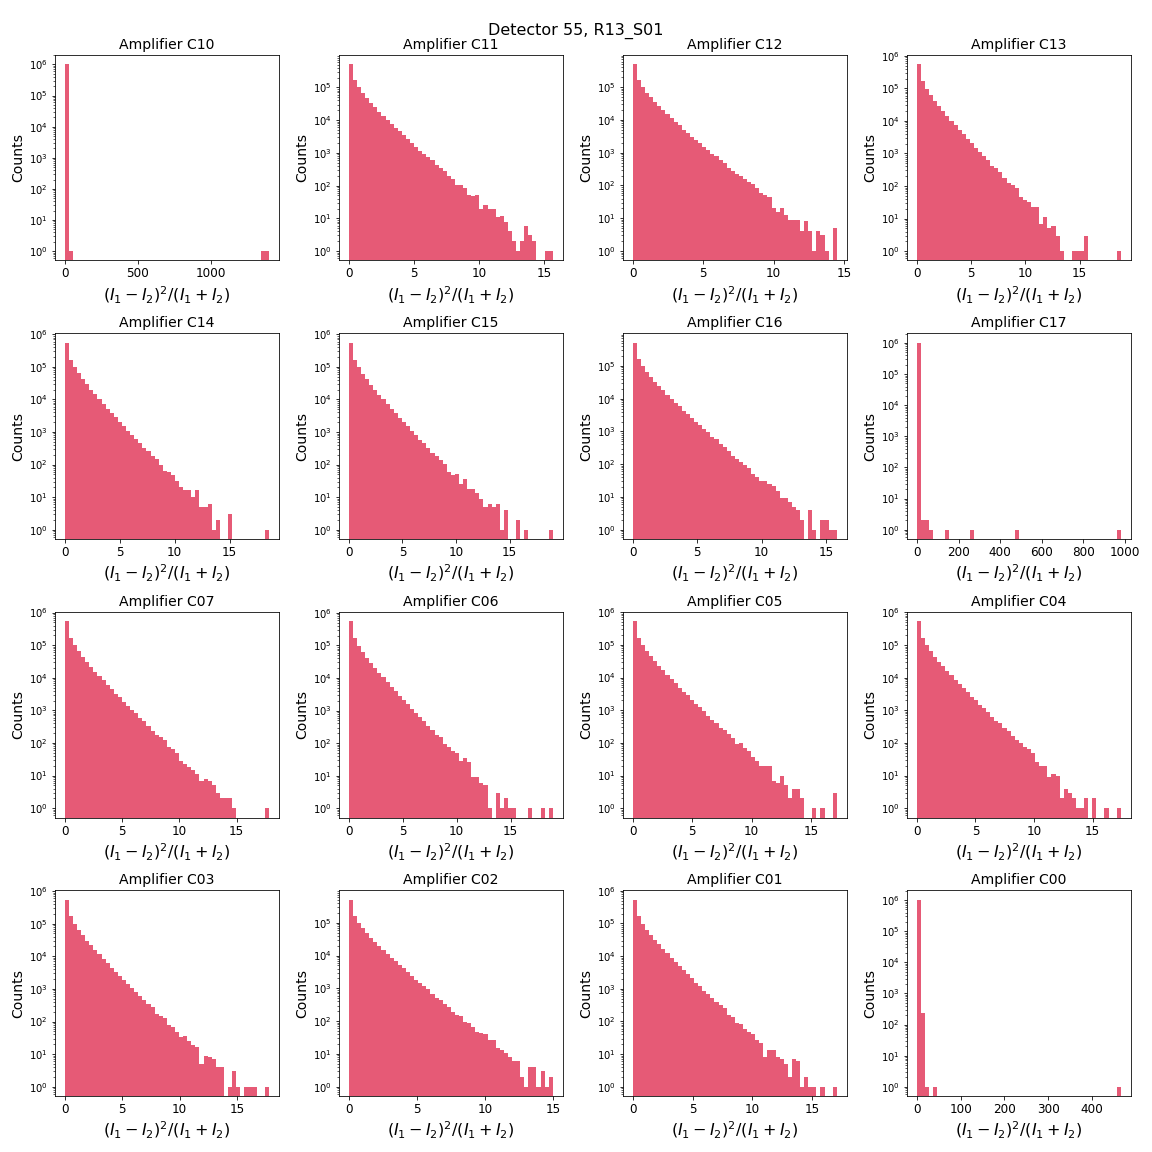
\includegraphics[width=\textwidth]{Figures/Histogram_ratioIM_det55.png}
    \caption{Histogram of the distribution for $\frac{(I_1 - I_2)^2}{I_1 + I_2}$ for each segment of detector 55 (R13\_S01). }
    \label{fig:hist_ratioIM}
\end{figure}


\begin{figure}[!htb]
     \centering
     \begin{subfigure}[b]{\textwidth}
         \centering
         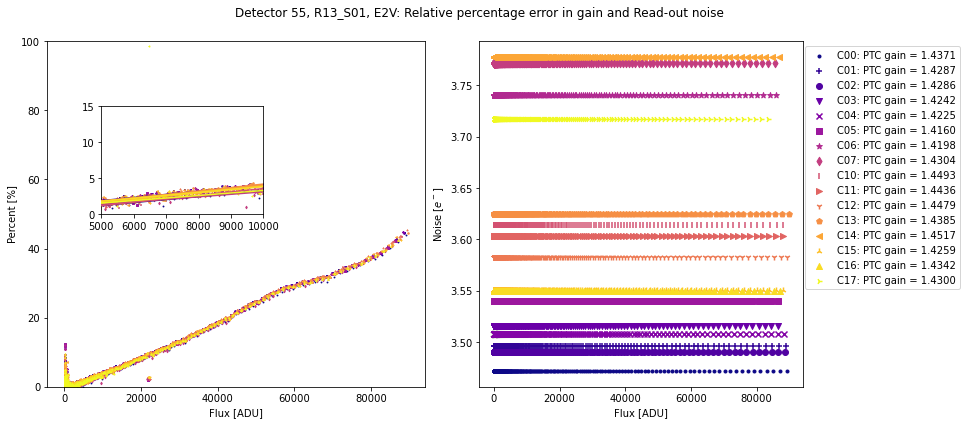
\includegraphics[width=\textwidth]{Figures/Relative_Error_Gain_Noise_detectorR13_S01.png}
     \end{subfigure}
     \vspace{3mm}
     \begin{subfigure}[b]{\textwidth}
         \centering
         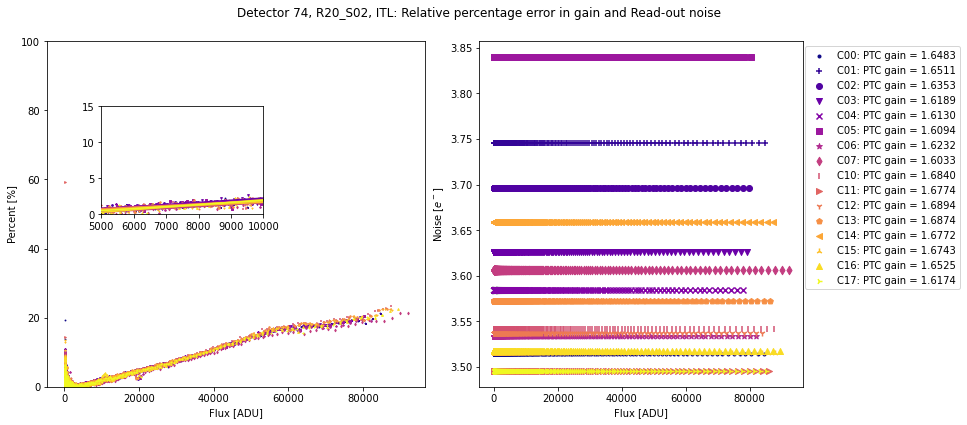
\includegraphics[width=\textwidth]{Figures/Relative_Error_Gain_Noise_detectorR20_S02.png}
     \end{subfigure}
        \caption{Refer to the description of the figure \ref{fig:relative_error_oldcode}. This plot uses the updated code (version w\_2022\_32) that does not use clipped mean.}
        \label{fig:relative_error}
\end{figure}

\begin{figure}[!htb]
     \centering
     \begin{subfigure}[b]{\textwidth}
         \centering
         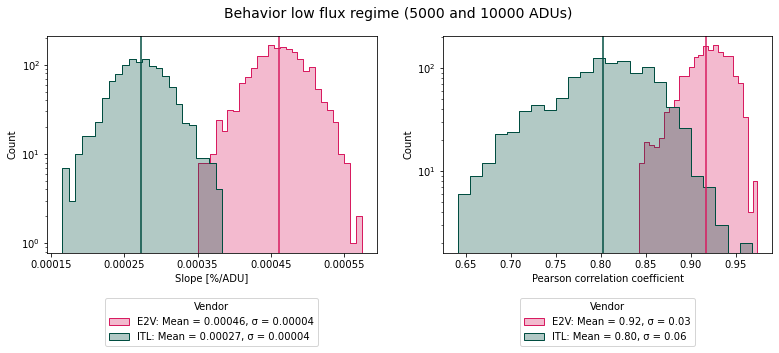
\includegraphics[width=\textwidth]{Figures/Histogram_slope_corr_new.png}
     \end{subfigure}
     \vspace{3mm}
     \begin{subfigure}[b]{\textwidth}
         \centering
         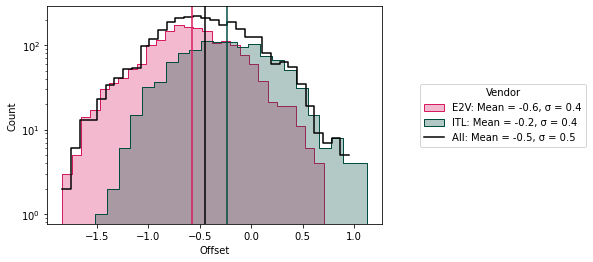
\includegraphics[width=0.7\textwidth]{Figures/Histogram_offset_new.png}
     \end{subfigure}
        \caption{Histograms for the slope (top left), Pearson's correlation coefficient (top right), and the y-axis intercept (offset, bottom panel) corresponding to the linear fit performed in the flow region between 5000 and 10000 ADU for the gain. Its construction used the updated code (version w\_2022\_32), and the colors represent the vendor, E2V in red and ITL in blue. The vertical lines represent the mean for each case.  }
        \label{fig:histogram_linearfit}
\end{figure}

\subsection{Crosstalk and non linearity correction} \label{subsec:crosstalk_and_linearity}

A part of the final analyses we performed during this internship consisted of quantifying and deciding whether the crosstalk effect and the nonlinearity impact the shape of the PTC and/or the fundamental parameters: gain, read noise, B-F effect, and turnoff coefficient.
%Parte de los análisis finales que efectuamos durante esta pasantía consistió en cuantificar y decidir si el efecto de crosstalk y la no linealidad tienen impacto en la forma de la PTC y/o de los parámetros fundamentales: ganancia, ruido de lectura, coeficiente del B-F effect y turnoff. 

\vspace{3mm}

As described in section \ref{subsec:method_Crosstalk}, we had access to the crosstalk matrices for detector 32 (ITL) and 139 (E2V), which are shown in Figure \ref{fig:crosstalk_matrix}. We obtained from applying the methodology of that section that the differences between PTC with and without crosstalk correction are shallow, as shown in Figure \ref{fig:crosstalk_corr32} and Figure \ref{fig:crosstalk_corr139}. They illustrated that considering the region below saturation, the difference between the variances is consistently below 0.1 ADU. In contrast, the most significant variance in the parameters is $\sim 0.1$\% in read noise and BF effect coefficient and  $\sim 0.07$ \% in gain and turnoff. The most significant differences were found in the ITL detector segments. According to the above, we conclude that the crosstalk does not have a considerable effect. So, correcting this effect is unnecessary since the difference in the parameters is small and does not alter the shape of the PTC.  

%Como se describió en la sección \ref{subsec:method_Crosstalk}, tuvimos acceso a las matrices de crosstalk para el detector 32 (ITL) y el 139 (E2V), que se muestran en las figura \ref{fig:crosstalk_matrix}. Como resultado de la metodología de dicha sección obtuvimos que las diferencias de la PTC corregida y no corregida por crosstalk es muy baja, como se muestra en las figura \ref{fig:crosstalk_corr32} y \ref{fig:crosstalk_corr139}, donde se muestra que considerando la región por debajo de saturación, la diferencia entre las varianzas está por debajo siempre de 0.1 ADU, mientras que en los parámetros la mayor variación es de $\sim 0.1$\% en el ruido de lectura y en el coeficiente del B-F effect y $\sim 0.07$ \% en la ganancia y el turnoff. Las mayores diferencias se encontraron en los segmentos del detector de ITL. De acuerdo con lo anterior, llegamos a la conclusión de que el crosstalk no tiene un efecto importante y no es necesario corregir por este efecto ya que la diferencia en los parámetros es pequeña y no altera la forma de la PTC.  



\begin{figure}[!htb]
    \centering
    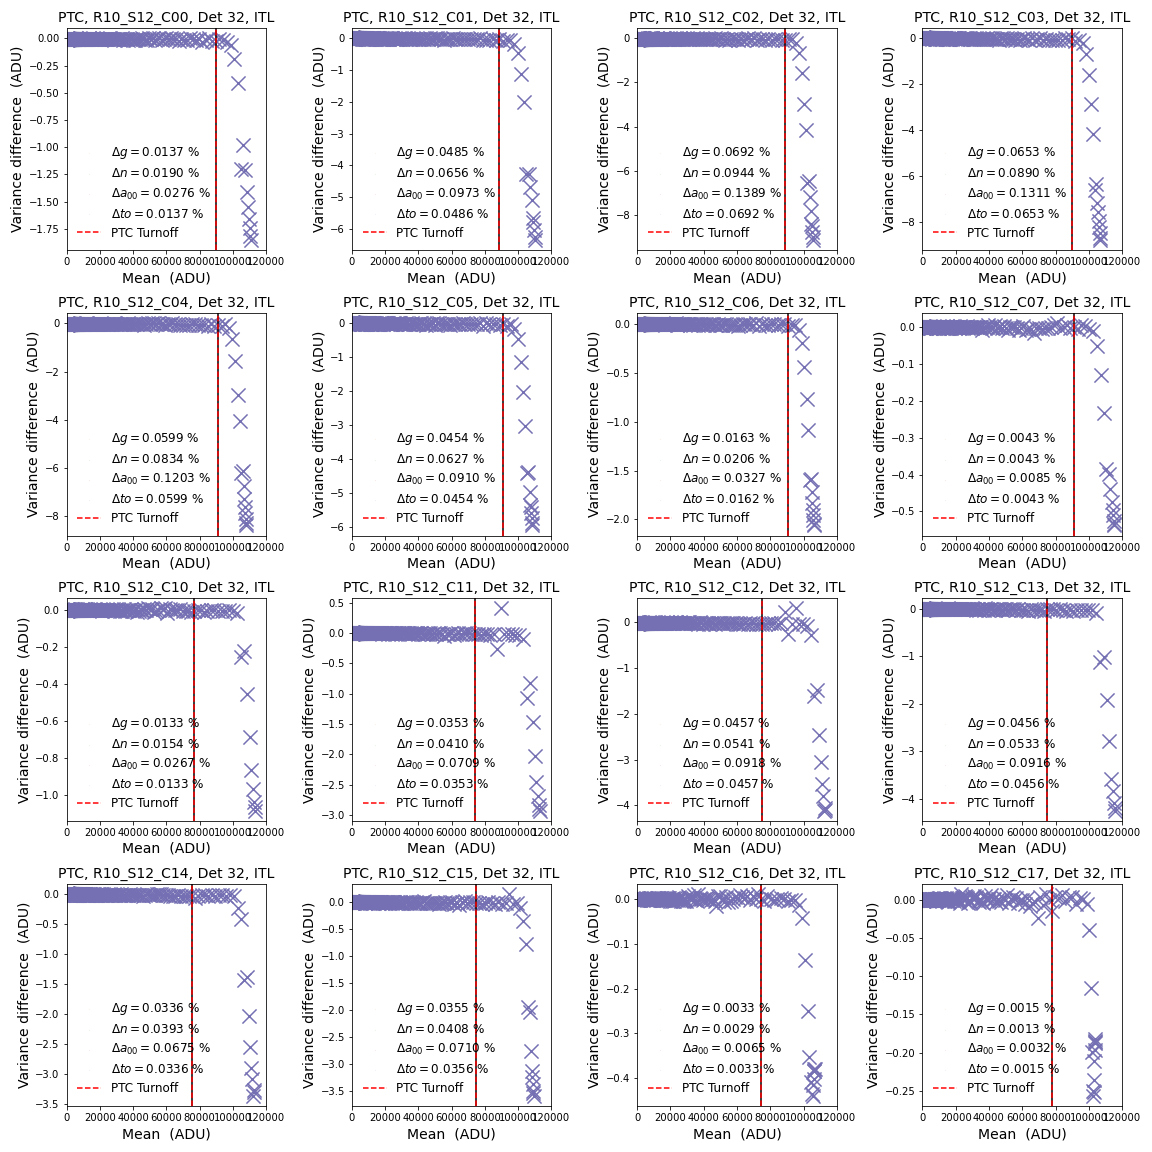
\includegraphics[width=\textwidth]{Figures/ptc_crosstalk32.png}
    \caption{The plot of the variance difference vs. mean for detector 32 (R10\_S12) for vendor ITL, where the variance difference is between the variance value without and with crosstalk correction. This is shown for each CCD segment, where the vertical lines mark the  PTC-turnoff values. In the legends, we displayed the differences between the parameters:  $\Delta g$ for the gain, $\Delta n$ for the read noise, $\Delta a_{00}$ for the brighter-fatter effect coefficient, and $\Delta to$ for the PTC-turnoff.}
    %Gráfica de la diferencia de varianza vs la media para el detector 32 (R10\_S12) para el fabricante ITL, donde la diferencia de varianza es entre el valor de varianza sin y con corrección por crosstalk. Se muestra esto para cada uno de los segmentos del CCD, mostrando por la línea vertical los valores de PTC-turnoff y en las respectivas leyendas las diferencias entre los parámetros: $\Delta g$ para la ganancia, $\Delta n$ para el ruido de lectura, $\Delta a_{00}$ para el coeficiente del brigther-fatter effect y $\Delta to$ para el PTC-turnoff.}
    \label{fig:crosstalk_corr32}
\end{figure}

\begin{figure}[!htb]
    \centering
    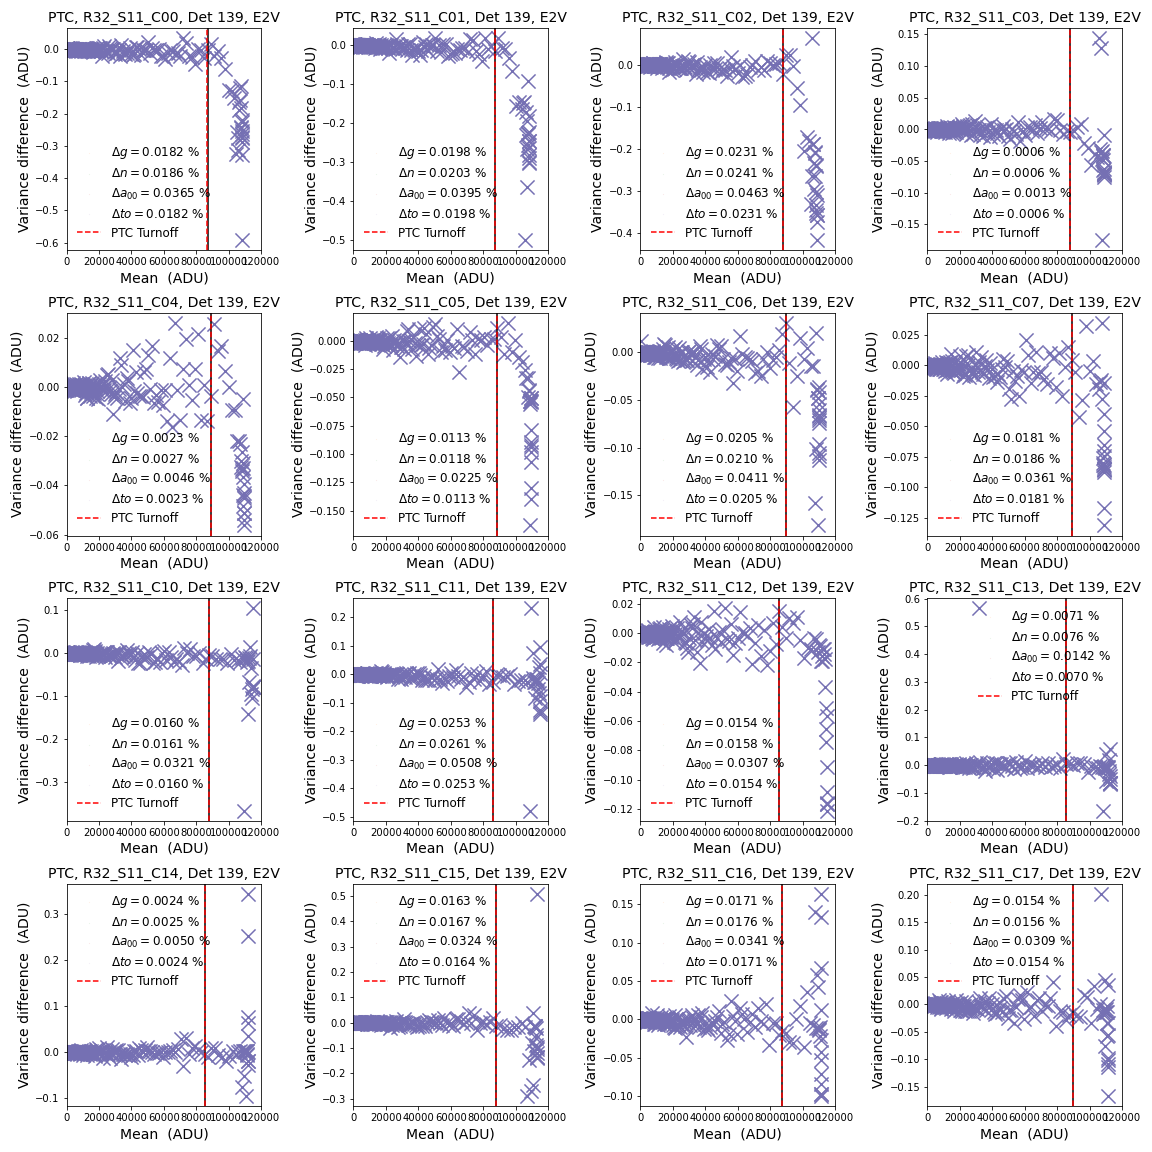
\includegraphics[width=\textwidth]{Figures/ptc_crosstalk139.png}
    \caption{Refer to the description of the figure \ref{fig:crosstalk_corr32}. This plot is for detector 139 (R32\_S11) for vendor E2V.}
    \label{fig:crosstalk_corr139}
\end{figure}

Finally, the 12-node cubic spline linearizer was applied to verify its impact on the PTC shape. The result of correcting only for crosstalk (orange dots), only for nonlinearity (blue diamonds), corrected for both effects (gray triangles), and the uncorrected data (magenta squares) is presented in Figure \ref{fig:varmean_crosstalk}. We see that the uncorrected data show a bump around 60000 ADU, while the crosstalk-corrected data are always located at the same position as the uncorrected data (thus also showing the bump),the data corrected for nonlinearity flatten it. Accordingly, making both corrections to the data has no more significant effect than fixing for nonlinearity alone. Again we find that the crosstalk is not a necessary correction since it does not affect either the shape or the parameters of the PTC. 

%Finalmente, se aplicó el linealizador spline cúbico de 12 nodos para verificar su impacto en la forma de la PTC. Se presenta en la figura \ref{fig:varmean_crosstalk} el resultado de corregir solo por crosstalk (puntos naranja), solo por la no linealidad (diamantes azules), corregidos por ambos efectos (triángulos grises) y los datos sin corregir (cuadrados magenta). Vemos que los datos sin corregir presentan un bache alrededor de los 60000 ADU, mientras que los datos corregidos por crosstalk se ubican siempre en la misma posición de los datos no corregidos (por tanto también muestran el bache), los datos corregidos por la no linealidad lo aplanan. De acuerdo con lo anterior, hacer las dos correcciones a los datos no tiene mayor efecto al que se obtiene corrigiendo solamente por la no linealidad. Nuevamente comprobamos que el crosstalk no es una corrección necesaria dado que no afecta ni la forma, ni los parámetros de la PTC. 


\begin{figure}[!htb]
     \centering
     \begin{subfigure}[b]{0.49\textwidth}
         \centering
         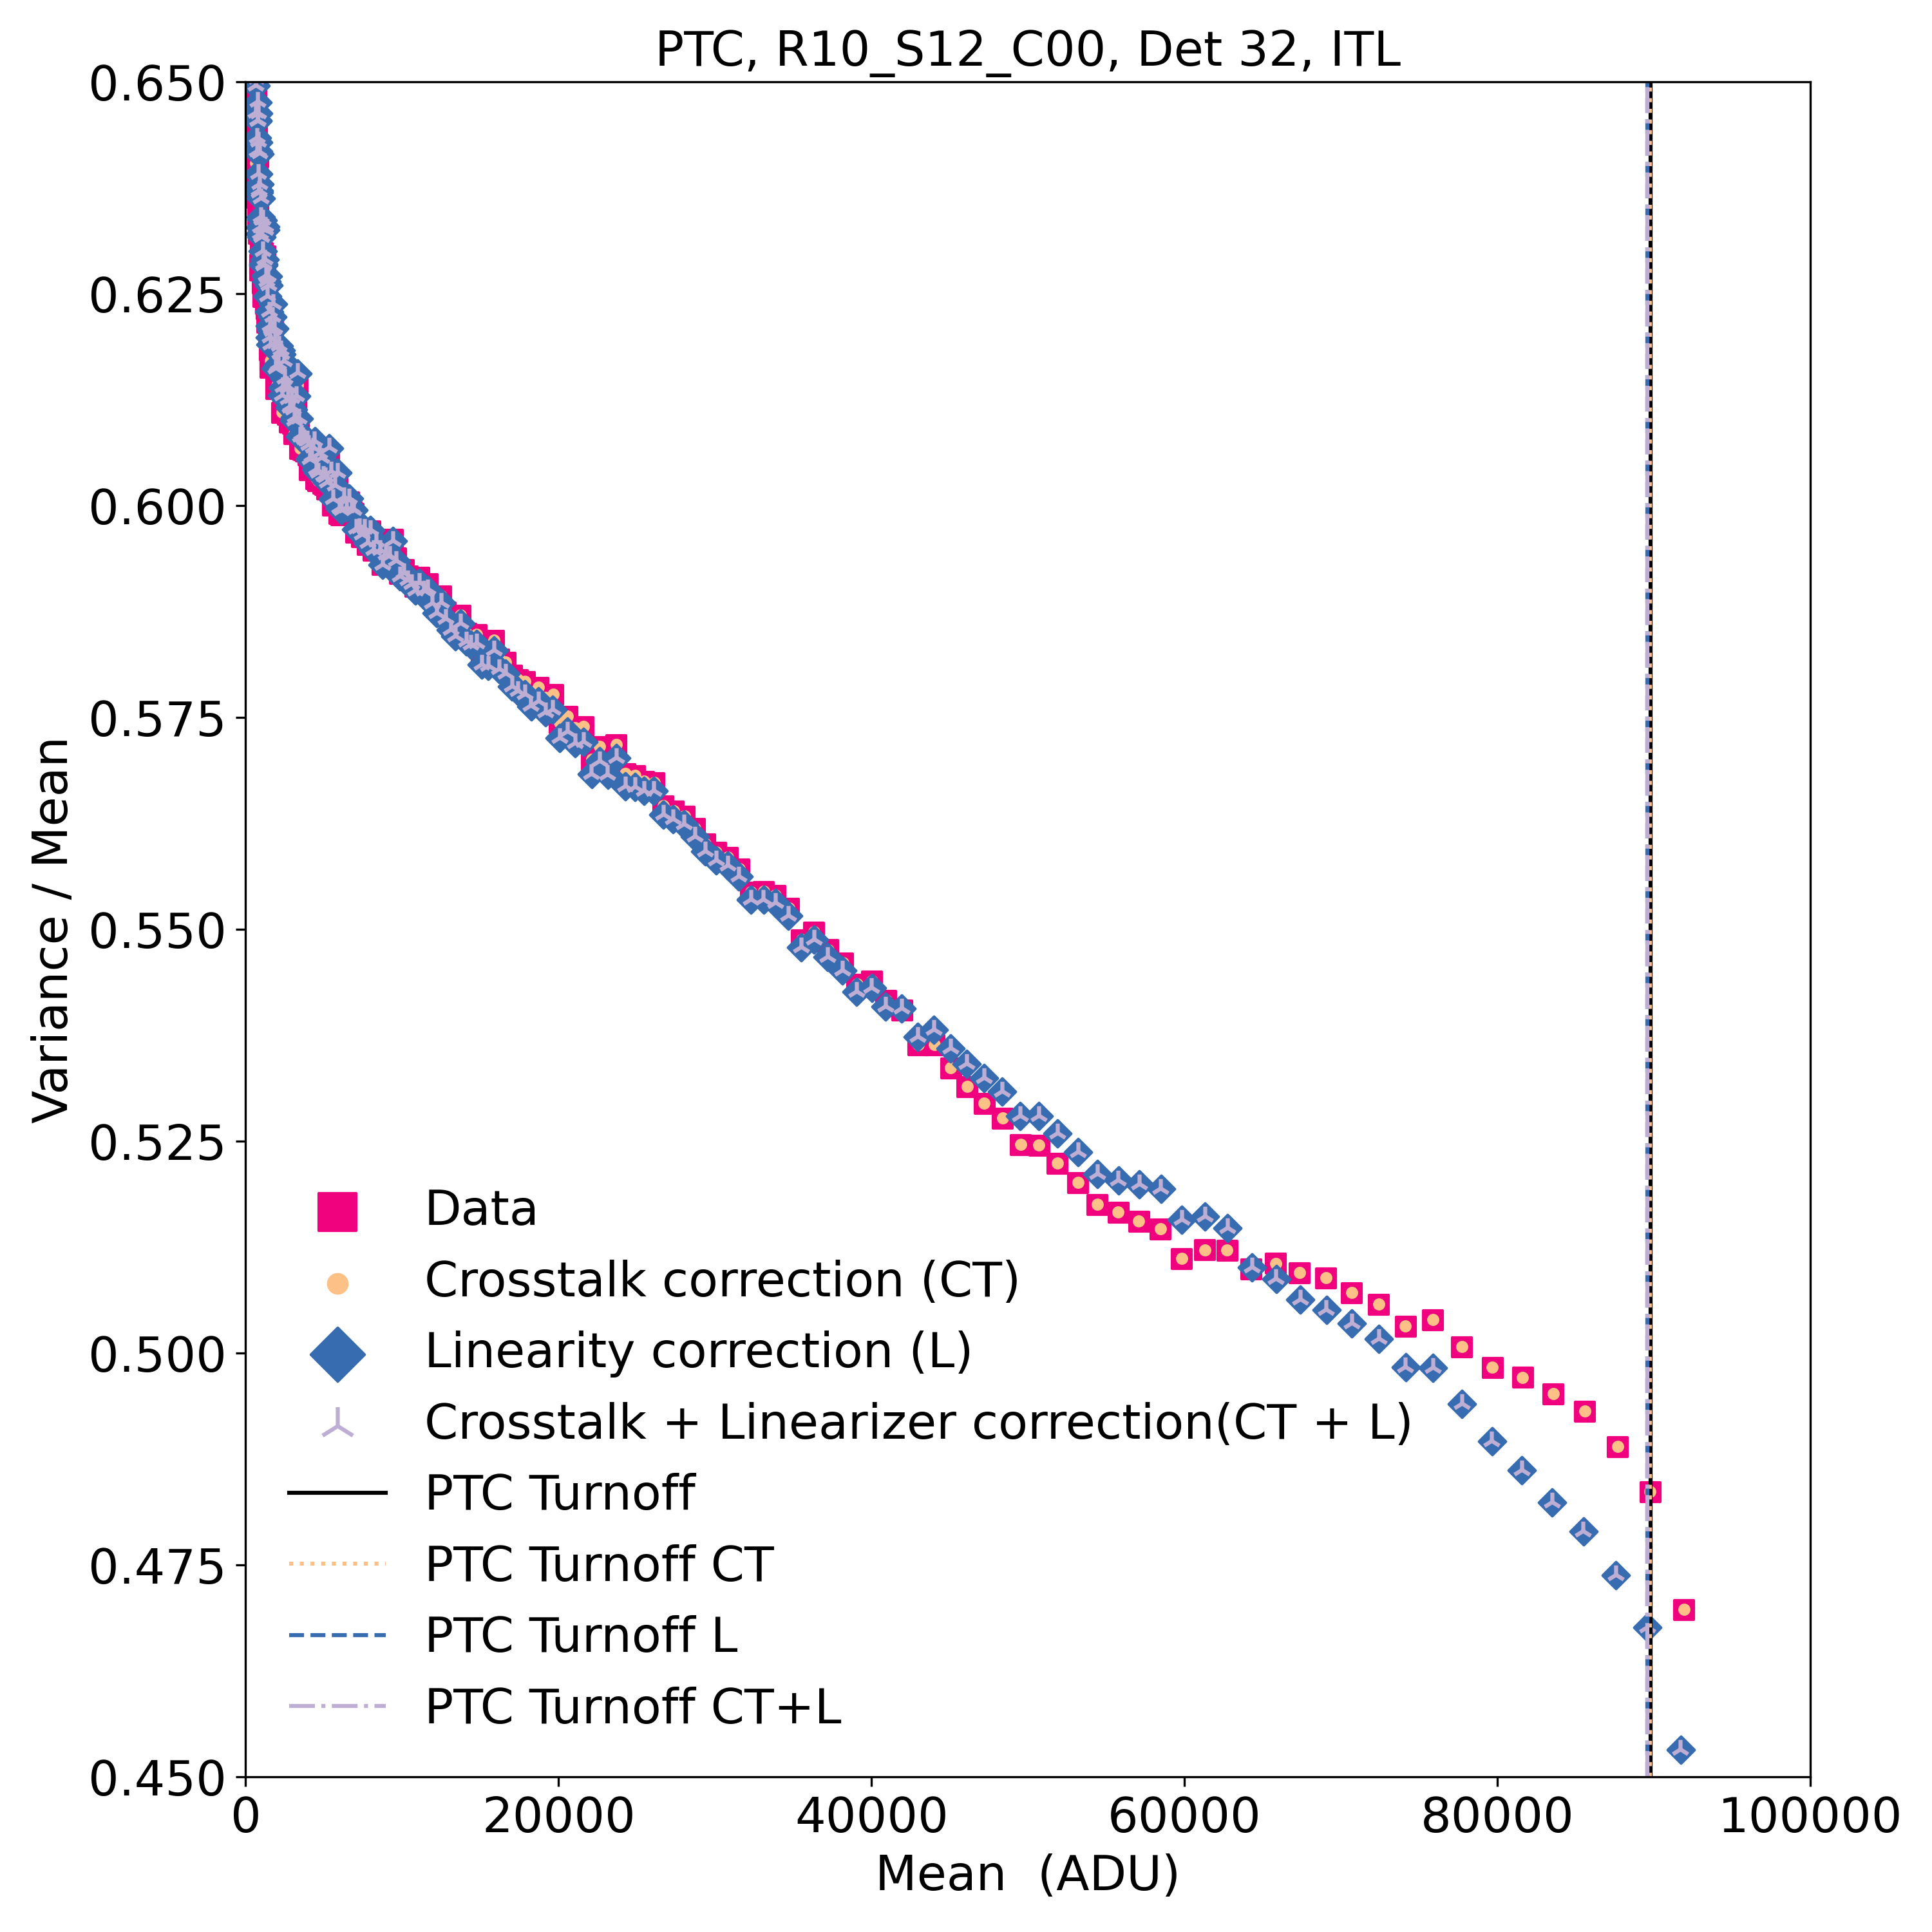
\includegraphics[width=\textwidth]{Figures/Variance_Mean_vs_Mean32.png}
     \end{subfigure}
     \hfill
     \begin{subfigure}[b]{0.49\textwidth}
         \centering
         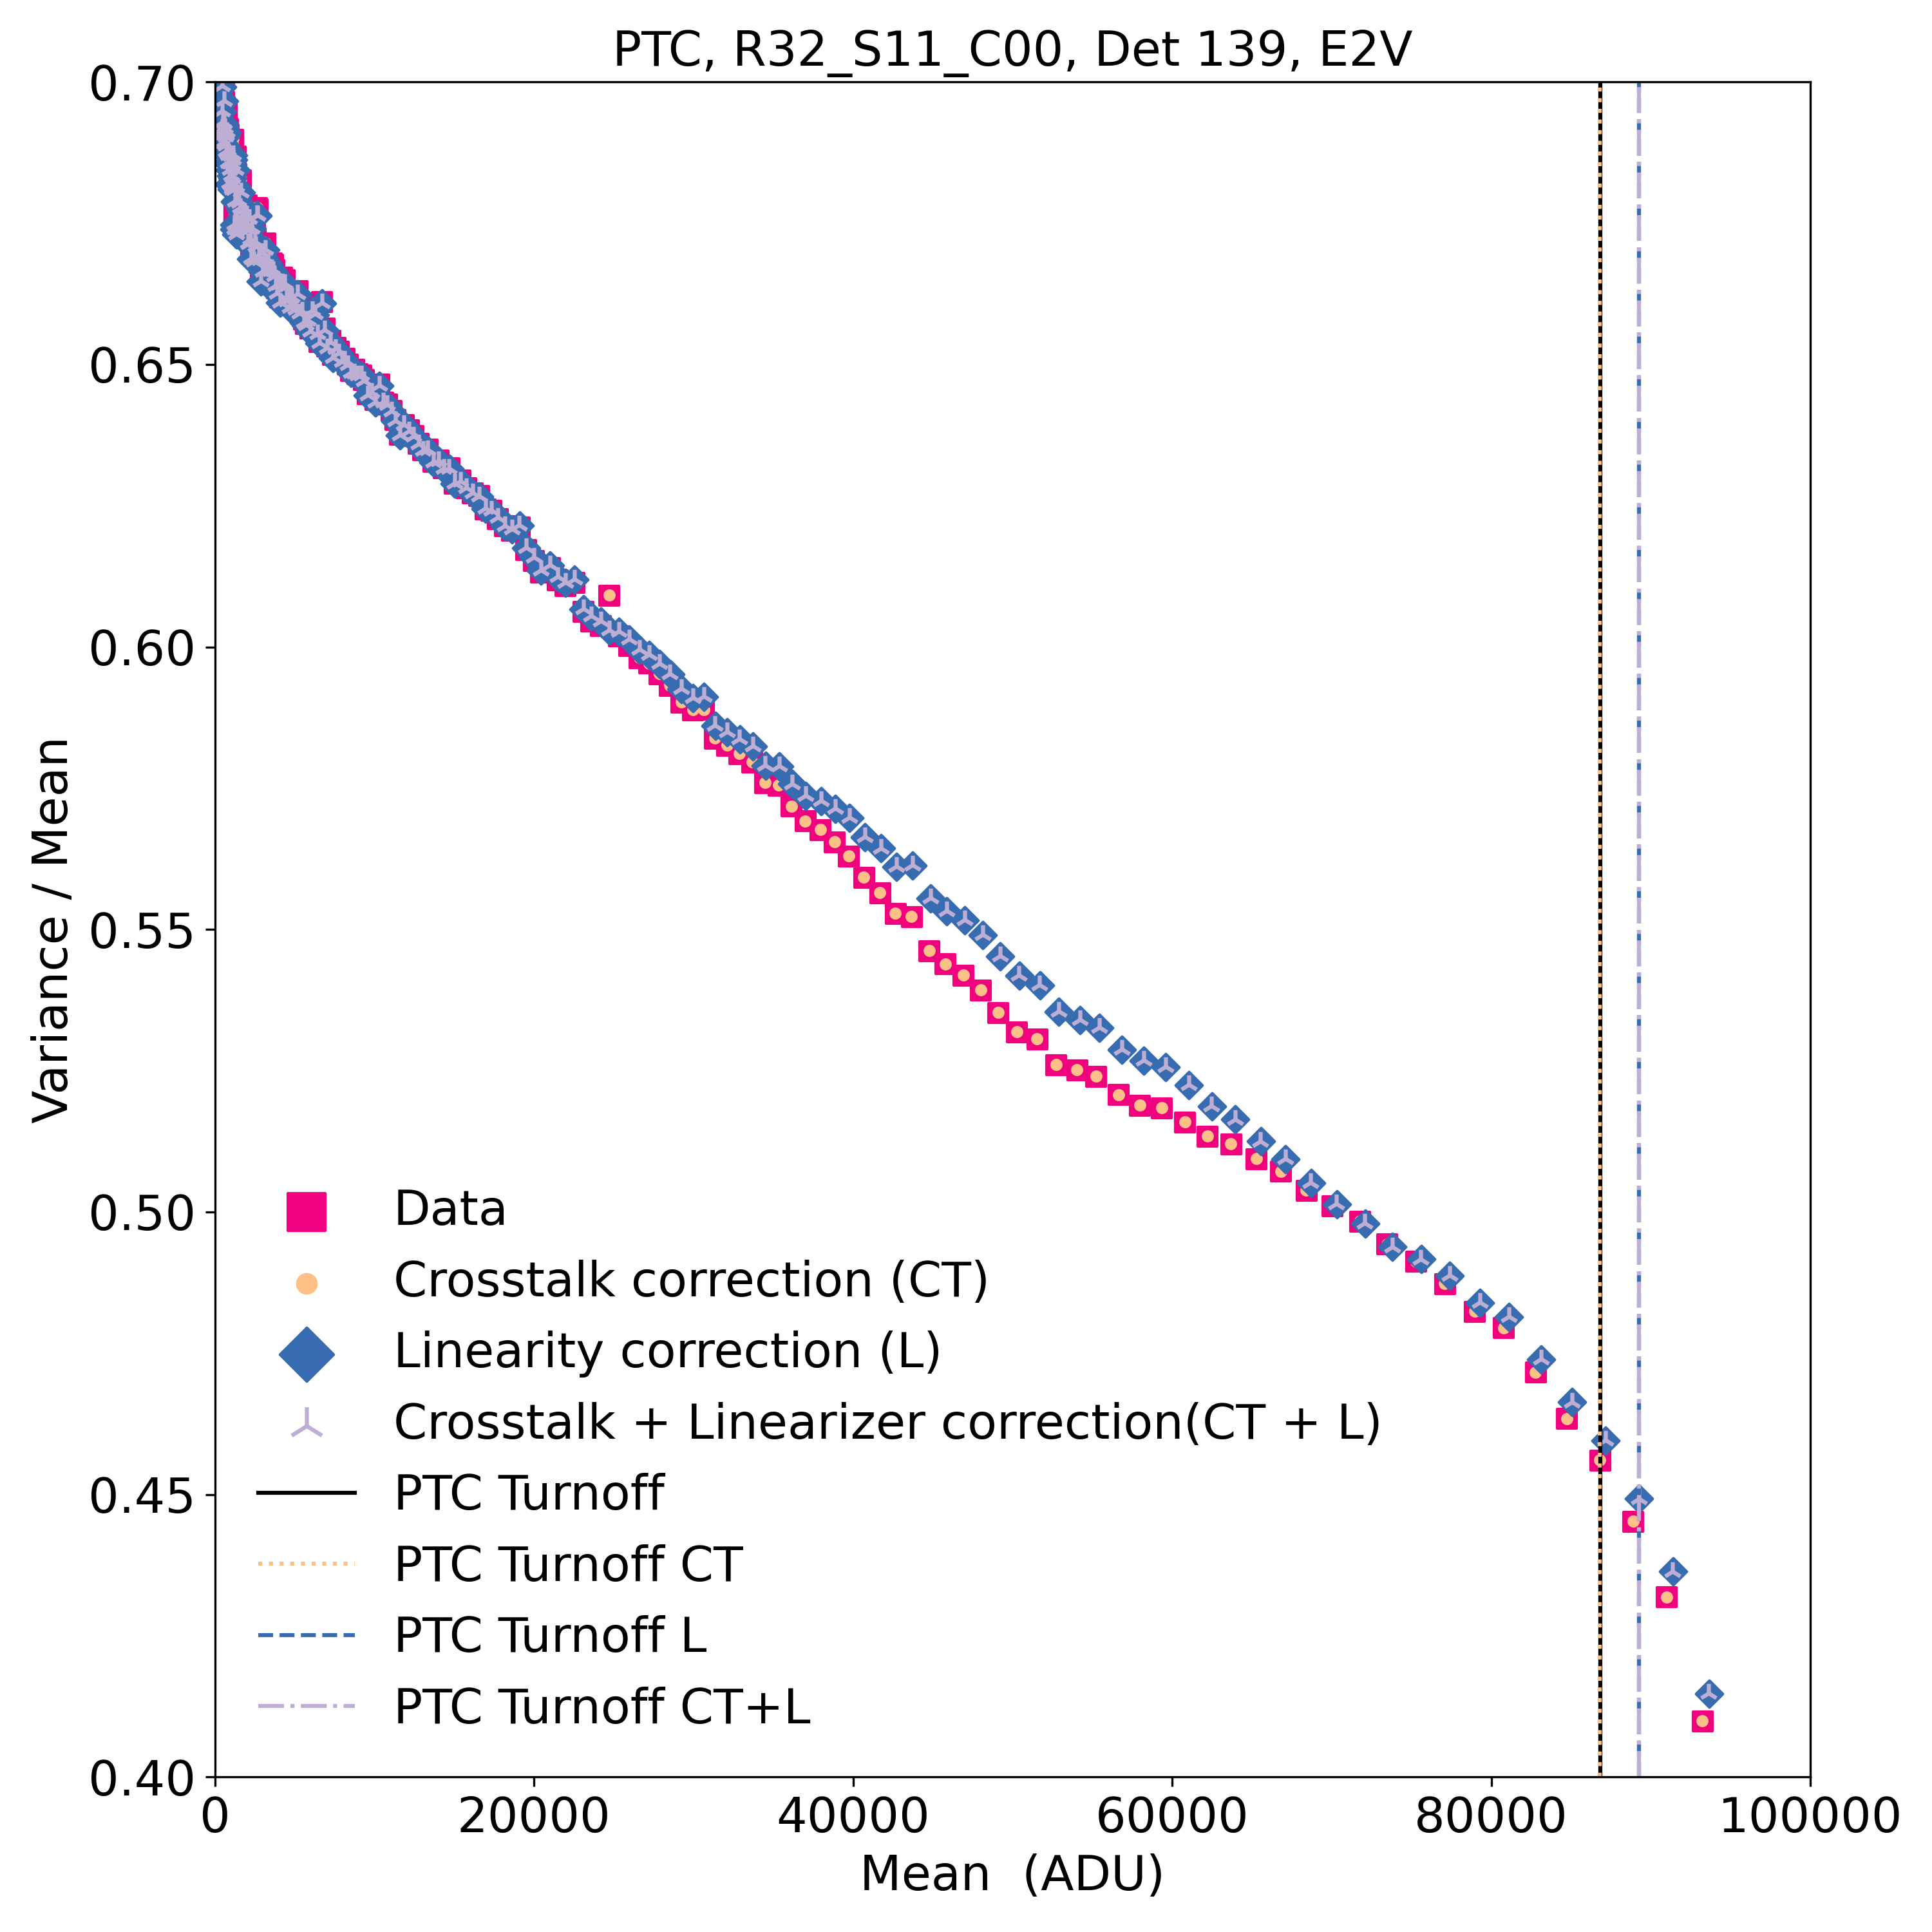
\includegraphics[width=\textwidth]{Figures/Variance_Mean_vs_Mean139.png}
     \end{subfigure}
        \caption{Variance normalized by mean vs. mean, for detector 32 (R10\_S12) for vendor ITL, on the left, and for detector 139 (R32\_S11) for vendor E2V, on the right. We show the data with no correction by crosstalk (CT) and nonlinearity in magenta squares. The orange dots show the data corrected for CT. The data corrected for nonlinearity with blue diamonds. Also, the triangles for data with corrections by both effects: TC and nonlinearity. Finally, the vertical lines represent the location of the turnoff.}
        
        %Varianza normalizada por la media vs la media, del detector 32 (R10\_S12) para el fabricante ITL, a la izquierda, y para el detector 139 (R32\_S11) del fabricante E2V, a la derecha. Se muestra en cuadrados magenta los datos sin corregir por crosstalk (CT) o por la no linealidad, en punto naranja los datos corregidos por CT, por lo diamantes azules los datos corregidos por la no linealidad y por los triángulos los datos corregidos por estos dos efectos: CT y no linealidad. Las líneas verticales representan la ubicación del turnoff.}
        \label{fig:varmean_crosstalk}
\end{figure}


\cite{scipy_2020}
\section{Conclusions} \label{sec:conclusions}

We present in this report a list of the sensors that present differences in the parameters with those obtained by SLAC, a PTC with low turnoff, and an inadequate classification of the same so that they can be reviewed later. We use the default value to determine the turnoff via \textit{DM stack}: decrease by at least 2 points to indicate shutdown.

\vspace{3mm}

We find in the PTC study that there is a bimodality per vendor for gain and $a_{00}$ and a more generalized behavior for read noise and turnoff. The average value we found for the gain in the E2V sensors of $1.49 \pm 0.05$ and $1.69 \pm 0.05$ $e^{-}/ADU$ for ITL. The coefficient of the BF effect has an average value of $(-3.0 \pm 0.1)\times 10 ^{-6}$ and $(-1.7 \pm 0.2)\times 10 ^{-6}$ for E2V and ITL, respectively. In addition, ITL detectors present a higher read noise dispersion compared to E2V ($6.7 \pm 1.0 \; e^{-}$ and $5.4 \pm 0.2 \; e^{-}$, respectively). The results obtained in this work are generally congruent with those obtained by SLAC. However, the main difference was observed in the Full Well Capacity value: in this work, we found a value of $130000 \pm 10000$ e$^-$, while SLAC a value of $90000$ e$^-$, which is a product of the different ways of calculating the turnoff between \textit{eotest} and \textit{DM stack}.

\vspace{3mm}

The analysis between the gain obtained from a pair of flats and the gain obtained from the PTC initially yielded a relative percentage error for low fluxes (5K and 10K ADU) higher than 5\%. This result led to a thorough investigation of its origin, finding that the distribution following the Lupton equation for flat images is not of Gaussian type, so the truncation of the distribution to calculate the statistics generating a shift of the mean value, and consequently, larger values of gain concerning the PTC gain. Therefore, this calculation was performed without truncation and obtained percentage differences between these two gains of $(1.8 \pm 0.7, 4.1 \pm 0.9)$ for E2V and $(0.85 \pm 0.7, 2.2 \pm 0.9)$ for ITL, where these intervals correspond to a flow region between 5000 and 10000 ADU. Consequently, the respective report was made and finally implemented in the main code. 


\vspace{3mm}

Finally, the linearity correction fixes the observed bump around 50K-60K ADU. Whereas performing a correction for crosstalk does not affect the shape of the PTC, nor does it significantly modify the parameters. Therefore, we recommend correcting for linearity only.  


\section{Acknowledgments} \label{sec:acknowledgments}


I would like to express my sincere gratitude to the entire RECA internship program team for their vision and efforts in creating this program that has provided an invaluable opportunity for research and learning for students in Colombia. I am also grateful to LSSST Corporation for generously supporting the realization of this project.

I am deeply thankful to my advisors, Drs. Andrés M. Plazas and Craig Lage, for their guidance, mentorship, and unwavering support throughout this learning journey. Their expertise, patience, and willingness to address my questions have been instrumental in shaping the outcomes of this project. Despite the challenges of virtual collaboration, their dedication and mentorship have fostered a close relationship that I deeply appreciate.

I would also like to acknowledge my colleague Jerónimo Calderón for the engaging discussions, valuable feedback, and camaraderie during the course of this project.

Finally, I am grateful to all other individuals, including fellow researchers and collaborators, who have provided assistance, advice, and encouragement during this project. Your support has been invaluable in the completion of this work.


\appendix
% Include all the relevant bib files.
% https://lsst-texmf.lsst.io/lsstdoc.html#bibliographies
\section{References} \label{sec:bib}
\renewcommand{\refname}{} % Suppress default Bibliography section
\bibliography{local,lsst,lsst-dm,refs_ads,refs,books}

% Make sure lsst-texmf/bin/generateAcronyms.py is in your path
\section{Acronyms} \label{sec:acronyms}
\addtocounter{table}{-1}
\begin{longtable}{p{0.145\textwidth}p{0.8\textwidth}}\hline
\textbf{Acronym} & \textbf{Description}  \\\hline
ADU & Analog-to-Digital Unit    \\
AGN & Active Galactic Nuclei    \\
BAO & Baryonic Acoustic Oscillations    \\
BF & Brighter Fatter    \\
BOT & Bench for Optical Testing    \\
BPS & Batch Processing Service    \\
CCD & Charge-Coupled Device    \\
CDF & Cumulative Distribution Function    \\
DM & Data Management    \\
E2V & Teledyne e2V    \\
FWC & Full Well Capacity    \\
ISR & Instrument Signature Removal    \\
ITL & Imaging Technology Laboratories    \\
NEO & Near-Earth Object    \\
PDF & Probability Density Function    \\
PSF & Point Spread Functions    \\
PTC & Photon Transfer Curve    \\
RECA & Red de Estudiantes Colombiana de Astronomía (Colombian Student Network of Astronomy)\\
TNO & Trans-Neptunian Object    \\
\hline
\end{longtable}

% If you want glossary uncomment below -- comment out the two lines above
%\printglossaries





\end{document}